%===============================================================================
% $Id: ifacconf.tex 19 2011-10-27 09:32:13Z jpuente $  
% Template for IFAC meeting papers
% Copyright (c) 2007-2008 International Federation of Automatic Control
%===============================================================================
\documentclass[a4paper]{ifacconf}

\usepackage{graphicx,amsmath,url}      % Configura figuras 
\usepackage[round]{natbib}             % Configura bibliografia
%===============================================================================


% ===============================================================
% Choose the language of the manuscript.
% If in English, choose 
% \def\portugues{0} 
%
% If in Portuguese or Spanish, choose
% \def\portugues{1} 
%
% Note that, if you are writing in Spanish, you need additional 
% adjusts in some parts of the text, which have been put in Portuguese only.
\def\portugues{1} 
% ===============================================================

% If the above line is commented, it is assumed manuscript in English:
\ifx\portugues\undefined
\def\portugues{0}
\fi


\if\portugues0
   \usepackage[english]{babel}
  \else
   \usepackage[brazil,english]{babel}
\fi

  

\usepackage[T1]{fontenc}
%\usepackage{inputenc}

\usepackage[utf8]{inputenc}

\usepackage{ae}


\if\portugues1
% =====================================================================
% =====================================================================
% If the manuscript is in Spanish, please change the texts adequatelly.
% You may also add other definitions in this part.
 \newtheorem{teorema}[thm]{{\em Teorema}}{ }
 \newtheorem{lema}[thm]{{\em Lema}}{ }
 \newtheorem{corolario}[thm]{{\em Corolário}}{ }
 \newenvironment{prova}{{\bf Prova.}}{ }
% ===============================================================
\fi

\usepackage{xcolor}
\usepackage{tikz}
\usetikzlibrary{arrows.meta,angles,quotes}
% Permite quebrar URLs longas na bibliografia
% Permite quebrar URLs longas na bibliografia
\usepackage{xurl}

% Permite quebrar URLs longas na bibliografia
\usepackage{xurl}

% Preserva a definição original da classe IFAC
\makeatletter
\let\IFACOriginalSsect\@ssect
\makeatother

% Habilita hyperlinks sem bordas coloridas
\usepackage[hidelinks]{hyperref}

% Compatibilidade dos marcadores PDF com a classe IFAC
\providecommand*{\theHpart}{0}

% Restaura a formatação original dos títulos sem numeração
\makeatletter
\let\@ssect\IFACOriginalSsect
\makeatother

% Padroniza a fonte das URLs
\urlstyle{same}

\usepackage[T1]{fontenc}
\usepackage[utf8]{inputenc}
\usepackage{lmodern}

% Largura do bloco Abstract/Resumo/Palavras-chave (padrão da classe: .8\textwidth)
% e correção do limite de altura do frontmatter na 1ª página (a classe usava
% um valor ~100pt menor que \textheight, empurrando as palavras-chave para a pág. 2)
\makeatletter
\def\@abstractwidth{.85\textwidth}
\AtBeginDocument{\t@xtheight\textheight \advance\t@xtheight-\splittopskip}
\makeatother


\begin{document}
	
	
\if\portugues1

% =====================================================================
% =====================================================================
% USE THIS PART IF THE TEXT IS IN PORTUGUES OR SPANISH
% =====================================================================
% If the manuscript is in Spanish, please change the texts adequately.
% =====================================================================
% 
\selectlanguage{brazil}
	
\begin{frontmatter}

\title{Integração e validação da plataforma experimental autônoma VIDA por meio de fusão sensorial e controle de trajetória} 
% Title, preferably not more than 10 words.


\author[First]{Whilker Henrique Dos Santos Silva} 
\author[Second]{Danilo Alves De Lima} 


\address[First]{Escola de Engenharia - Departamento de Automática, Universidade Federal de Lavras (e-mail: whilker.silva@estudante.ufla.br).}
\address[Second]{Escola de Engenharia - Departamento de Automática, Universidade Federal de Lavras (e-mail: danilo.delima@ufla.br)}



\selectlanguage{english}
\renewcommand{\abstractname}{{\bf Abstract:~}}
\begin{abstract}                % Abstract of not more than 250 words.
Autonomous vehicle research requires extensive applied knowledge and experimental capabilities, often limited by access to affordable testing platforms. Commercial vehicles designed for this purpose are expensive and difficult to access, hindering research progress and the training of qualified professionals. To address this challenge, the Land Mobility Laboratory (LMT) at the Federal University of Lavras (UFLA) is developing the Intelligent Vehicle for Applied Development (VIDA), a small-scale electric vehicle for educational and scientific purposes. This work aims to integrate VIDA's subsystems into a unified architecture and validate it through an autonomous navigation task. The proposed solution employs a distributed computing architecture consisting of an ESP32 microcontroller, an Odroid N2 embedded computer, and a laptop, integrated through ROS 2. Low-level control employs proportional and integral (PI) actions for longitudinal velocity and proportional, integral, and derivative (PID) actions for steering. Localization combines measurements from wheel encoders, an LVDT sensor, an IMU, and a GNSS receiver with RTK corrections through an Extended Kalman Filter (EKF). Autonomous navigation is performed using the Stanley controller, incorporating curvature feedforward compensation and yaw-rate damping. Experimental validation involved two real-world routes, achieving lateral root mean square errors (RMSE) of 16.7 cm and 12.9 cm, respectively. The results demonstrate the feasibility of the developed architecture and the platform's ability to follow trajectories autonomously, establishing a foundation for future research on autonomous ground vehicles.



\vskip 1mm% não altere esse espaçamento
\selectlanguage{brazil}
{\noindent \bf Resumo}: O estudo de veículos autônomos requer amplo conhecimento aplicado e capacidade experimental muitas vezes limitadas à disponibilidade de uma plataforma de testes acessível. Veículos comerciais para esse propósito são caros e de difícil acesso, dificultando o avanço de pesquisas e formação de mão de obra especializada. É com esse intuito que o Laboratório de Mobilidade Terrestre (LMT) da Universidade Federal de Lavras (UFLA) está desenvolvendo o Veículo Inteligente de Desenvolvimento Aplicado (VIDA), um carro elétrico em escala reduzida para fins didáticos e científico. Este trabalho tem como objetivo realizar a integração dos subsistemas que compõem o VIDA em uma arquitetura unificada e validá-la por meio de uma tarefa de navegação autônoma. A solução proposta utiliza uma arquitetura computacional distribuída, composta por um microcontrolador ESP32, um computador embarcado Odroid N2 e um notebook, integrados por meio do framework ROS 2. O controle de baixo nível emprega ações proporcional e integral (PI) na velocidade longitudinal, e ações proporcional, integral e  derivativa (PID) no controle de esterçamento. Enquanto isso, a localização combina medições de sensores diversos, como encoders, LVDT, IMU e receptor GNSS com correções RTK, por meio de um filtro de Kalman estendido (EKF). A tarefa de navegação é realizada através controlador Stanley, incorporando compensação antecipativa de curvatura e amortecimento da velocidade angular. A validação experimental compreendeu dois percursos reais, nos quais foram obtidos os erros quadráticos médios em relação ao caminho desejado de 16,7 cm e 12,9 cm, respectivamente. Os resultados demonstram a viabilidade da arquitetura desenvolvida e a capacidade da plataforma de executar trajetórias autônomas, estabelecendo uma base para futuras pesquisas em veículos autônomos terrestres.
\end{abstract}

\selectlanguage{english}


\begin{keyword}
Autonomous vehicles; Trajectory tracking; Stanley controller; Sensor fusion.

\vskip 1mm
\selectlanguage{brazil}
{\noindent\it Palavras-chaves:} Veículos autônomos; Seguimento de trajetórias; Controlador Stanley; Fusão sensorial.
\end{keyword}


\selectlanguage{brazil}


\end{frontmatter}

% Restaura os hyperlinks internos desativados pelo modelo IFAC
\endNoHyper

\else
% ===============================================================
% ===============================================================
% USE THIS PART IF THE TEXT IS IN ENGLISH
% ===============================================================
% ===============================================================
% 

\begin{frontmatter}

\title{Style for SBA Conferences \& Symposia: Use Title Case for
  Paper Title\thanksref{footnoteinfo}} 
% Title, preferably not more than 10 words.

\thanks[footnoteinfo]{Sponsor and financial support acknowledgment
goes here. Paper titles should be written in uppercase and lowercase
letters, not all uppercase.}

\author[First]{First A. Author} 
\author[Second]{Second B. Author, Jr.} 
\author[Third]{Third C. Author}


\address[First]{Faculdade de Engenharia Elétrica, Universidade do Triângulo, MG, (e-mail: autor1@faceg@univt.br).}
\address[Second]{Faculdade de Engenharia de Controle \& Automação, Universidade do Futuro, RJ (e-mail: autor2@feca.unifutu.rj)}
\address[Third]{Electrical Engineering Department, 
   Seoul National University, Seoul, Korea, (e-mail: author3@snu.ac.kr)}
   
\renewcommand{\abstractname}{{\bf Abstract:~}}   
   
\begin{abstract}                % Abstract of not more than 250 words.
These instructions give you guidelines for preparing papers for IFAC
technical meetings. Please use this document as a template to prepare
your manuscript. For submission guidelines, follow instructions on
paper submission system as well as the event website.
\end{abstract}

\begin{keyword}
Five to ten keywords, preferably chosen from the IFAC keyword list.
\end{keyword}

\end{frontmatter}
\fi

%===============================================================================
%===============================================================================
%===============================================================================

\clearpage % Introdução começa sempre na página 2
\section{Introdução}
\label{sec:introducao}

O desenvolvimento de veículos autônomos tem despertado crescente interesse da indústria automobilística e da comunidade científica. No setor automotivo, esse interesse está associado à expansão do mercado de sistemas avançados de assistência ao condutor (\textit{Advanced Driver Assistance Systems} -- ADAS) e às perspectivas de desenvolvimento e comercialização de tecnologias com níveis mais elevados de automação. Segundo estimativas da McKinsey, o mercado global de software e componentes eletrônicos relacionados a essas tecnologias poderá alcançar aproximadamente US\$ 160 bilhões até 2035, com crescimento anual projetado de cerca de 16\% \citep{McKinsey2026}.

No âmbito científico, as pesquisas são motivadas pelo potencial dessas tecnologias para aumentar a segurança e a eficiência dos sistemas de transporte, bem como limitações nas metodologias de teste desses sistemas, particularmente na correspondência entre os resultados obtidos em simulação e o comportamento observado em ambientes reais \citep{Liao2025}.

No Brasil, diferentes grupos de pesquisa têm desenvolvido plataformas experimentais voltadas ao estudo de tecnologias de condução autônoma. Entre essas iniciativas, destacam-se os projetos CADU, da Universidade Federal de Minas Gerais (UFMG) \cite{Sabbagh2010}, CaRINA, da Universidade de São Paulo (USP) \cite{Fernandes2014}, e IARA, da Universidade Federal do Espírito Santo (UFES) \cite{Badue2021}. Essas iniciativas evidenciam o interesse da comunidade científica nacional pelo desenvolvimento e pela validação experimental de tecnologias aplicadas a veículos autônomos. 

Nesse contexto, o Laboratório de Mobilidade Terrestre (LMT), da Universidade Federal de Lavras (UFLA), iniciou em 2019 o desenvolvimento da plataforma VIDA (Veículo Inteligente de Desenvolvimento Aplicado). Trata-se de um veículo elétrico experimental concebido para apoiar pesquisas em automação e navegação de veículos terrestres \citep{Silva2024CIUFLA}.

Entre os desafios da condução autônoma, destaca-se o seguimento de trajetórias, que consiste em determinar as ações de controle necessárias para conduzir um veículo ao longo de um percurso de referência. Para isso, é necessária a integração entre os sistemas de localização e controle do veículo.

Diante desse cenário, este trabalho tem como objetivo implementar e validar experimentalmente um sistema de seguimento autônomo de trajetórias na plataforma VIDA, utilizando localização por fusão sensorial de encoders, sensor de esterçamento, giroscópio e receptor GNSS com correções RTK e controle lateral baseado no método Stanley.

A implementação envolve também o controle de baixo nível e uma arquitetura computacional distribuída baseada no ROS 2 (\textit{Robot Operating System 2}), composta por um microcontrolador ESP32, um computador embarcado Odroid e um notebook responsável por tarefas de alto nível. A validação é realizada mediante ensaios com o veículo real, considerando o acompanhamento da rota, os erros lateral e angular e o desempenho dos sistemas de controle.

Busca-se, assim, contribuir para a consolidação do VIDA como plataforma experimental para pesquisas futuras em veículos autônomos. Além da contribuição tecnológica e científica, o desenvolvimento deste trabalho também representa uma etapa importante na formação acadêmica em Engenharia de Controle e Automação, ao proporcionar a aplicação prática e integrada dos conhecimentos adquiridos ao longo da graduação.

Este artigo está estruturado da seguinte maneira: a Seção~\ref{sec:fundamentacao} apresenta a fundamentação teórica, enquanto a Seção~\ref{sec:plataforma} descreve a plataforma VIDA e seus principais subsistemas. Na Seção~\ref{sec:arquitetura}, é detalhada a arquitetura computacional adotada, seguida pela descrição dos controladores de baixo nível na Seção~\ref{sec:baixo_nivel}. As Seções~\ref{sec:estimacao} e~\ref{sec:seguimento_trajetoria} abordam, respectivamente, a estimação de estados e a implementação do seguimento de trajetórias. Por fim, a Seção~\ref{sec:resultados_experimentais} apresenta os resultados experimentais, e a Seção~\ref{sec:conclusao} reúne as conclusões do trabalho. 
\section{Fundamentação teórica}
\label{sec:fundamentacao}

O desenvolvimento de veículos inteligentes envolve a integração de diferentes conceitos relacionados à percepção do ambiente, à localização, ao planejamento de movimento e ao controle, sendo necessária uma arquitetura unificada e eficiente para executar todas as tarefas. Nesta seção, são apresentados os fundamentos teóricos necessários à compreensão da solução desenvolvida, abrangendo o modelo cinemático de bicicleta, o posicionamento GNSS (Sistema Global de Navegação por Satélite) com correções RTK (Cinemática em Tempo Real), a estimação de estados por filtro de Kalman estendido, o controle de trajetória pelo método Stanley \citep{Thrun2006}, além de exemplos de veículos autônomos e suas respectivas arquiteturas de sistema.

\subsection{Modelo cinemático de bicicleta}
\label{subsec:modelo_bicicleta}

A modelagem matemática do movimento de veículos terrestres permite descrever seu comportamento a partir das relações entre posição, orientação, velocidade e esterçamento. Entre as representações utilizadas para essa finalidade, destaca-se o modelo cinemático de bicicleta, que simplifica a geometria de direção Ackermann de um veículo de quatro rodas por meio de duas rodas equivalentes, posicionadas nos centros dos eixos dianteiro e traseiro \citep{Snider2009}. 

O modelo considera o movimento do veículo em um plano bidimensional, assumindo a condição derolamento sem deslizamento lateral dos pneus. Dessa forma, os efeitos dinâmicos associados às forças laterais, à transferência de carga e à interação entre os pneus e o solo, não são representados explicitamente. Essa aproximação é especialmente adequada para descrever o movimento de veículos em condições de baixa velocidade e manobras nas quais os efeitos de deslizamento lateral podem ser desprezados. 

Considerando um veículo com tração traseira e adotando o centro do eixo traseiro como ponto de referência, seu movimento pode ser descrito por:

\begin{equation}
\label{eq:modelo_cinematico}
\left\{
\begin{aligned}
\dot{x} &= v\cos(\theta) \\
\dot{y} &= v\sin(\theta) \\
\dot{\theta} &= \frac{v}{L}\tan(\delta)\\
\end{aligned}
\right.
\end{equation}

em que $x$ e $y$ representam as coordenadas da posição do veículo no referencial global, $\theta$ corresponde ao ângulo de orientação em relação a esse referencial, $v$ é a velocidade linear, $L$ representa a distância entre os eixos dianteiro e traseiro e $\delta$ corresponde ao ângulo de esterçamento equivalente das rodas dianteiras.

\begin{figure}[htb]
    \centering
    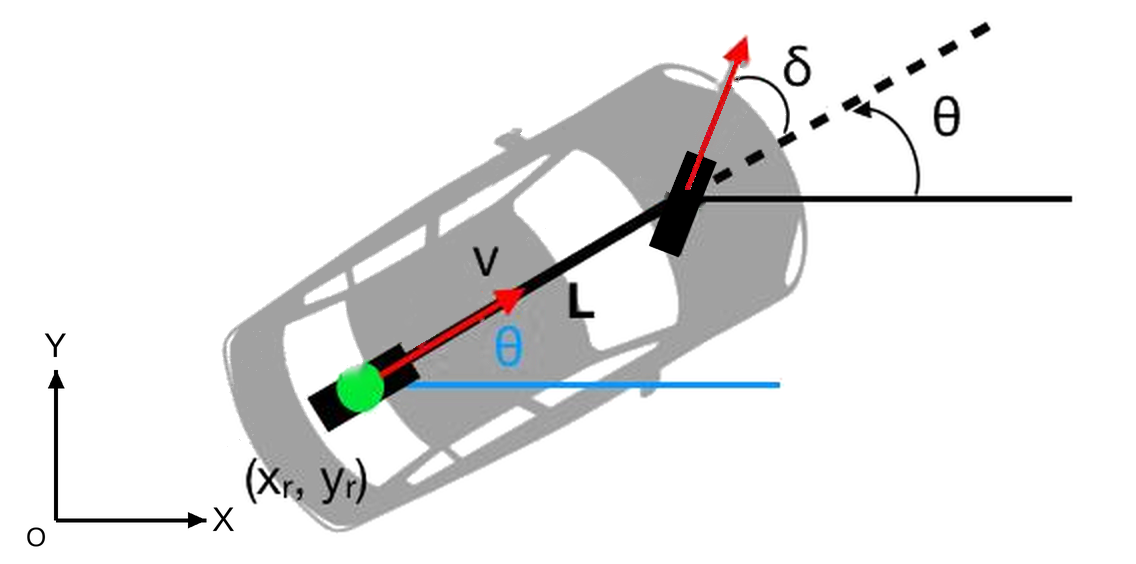
\includegraphics[width=0.85\columnwidth]{Imagens/Modelo cinemático de bicicleta.png}
    \caption{Representação geométrica do modelo cinemático de bicicleta. Fonte: \citet{Snider2009}.}
    \label{fig:modelo_bicicleta}
\end{figure}

As equações descrevem as velocidades de translação e de rotação do veículo em função da velocidade longitudinal e do ângulo de esterçamento. A partir da integração dessas relações ao longo do tempo, é possível determinar a evolução da posição e da orientação do veículo. Em particular, a taxa de variação da orientação depende diretamente da velocidade e da tangente do ângulo de esterçamento, sendo inversamente proporcional à distância entre os eixos \citep{Snider2009,Massera2014}. 

Embora simplificado, o modelo cinemático de bicicleta fornece uma representação matemática útil para o estudo da movimentação de veículos terrestres, constituindo uma base para o desenvolvimento de estratégias de localização, estimação de estados e controle de trajetórias.

\subsection{Posicionamento GNSS com RTK}

Os sistemas globais de navegação por satélite (\textit{Global Navigation Satellite Systems} -- GNSS) permitem determinar a posição de um receptor a partir de sinais transmitidos por diferentes constelações de satélites, como o GPS, dos Estados Unidos, o GLONASS, da Rússia, o Galileo, da União Europeia, e o BeiDou, da China. Entretanto, a precisão do posicionamento convencional é limitada por fatores como eerros orbitais e erros nos relógios dos satélites e dos receptores, atrasos atmosféricos e efeitos de multicaminhamento dos sinais. 
 
Para aplicações que exigem maior precisão, destaca-se a técnica RTK (\textit{Real-Time Kinematic}), baseada no posicionamento relativo entre um receptor móvel (\textit{rover}) e uma estação de referência com coordenadas conhecidas. A técnica utiliza observações da fase da portadora dos sinais GNSS e informações de correção para reduzir erros comuns às medições, possibilitando precisão centimétrica em condições favoráveis \citep{Bisnath2020}.  

A transmissão dessas correções pode ser realizada por meio do protocolo NTRIP (\textit{Networked Transport of RTCM via Internet Protocol}), que permite distribuir dados GNSS em tempo real pela internet. Nesse processo, as informações disponibilizadas por estações de referência são encaminhadas ao receptor móvel, permitindo a aplicação das correções durante o posicionamento \citep{BKG2026NTRIP}. 
 
A qualidade da solução RTK depende de fatores como a disponibilidade de sinais GNSS, a qualidade das observações e o recebimento adequado das correções. Entre os estados possíveis estão o RTK \textit{float}, no qual as ambiguidades da fase da portadora ainda não foram resolvidas como valores inteiros, e o RTK \textit{fixed}, no qual essa resolução foi obtida, permitindo maior precisão de posicionamento \citep{Ublox2025ZEDF9R}.

\subsection{Filtro de Kalman Estendido}
\label{subsec:fund_ekf}

A estimação de estados desempenha um papel fundamental em sistemas de navegação autônoma, uma vez que as medições dos sensores estão sujeitas a ruídos e incertezas. O filtro de Kalman é um estimador recursivo que combina informações de um modelo matemático com observações do sistema, considerando as incertezas associadas a ambas as fontes \citep{Welch2006}. 

O filtro de Kalman estendido (\textit{Extended Kalman Filter} -- EKF) permite aplicar essa abordagem a sistemas não lineares, por meio da linearização local dos modelos de movimento e observação por meio de matrizes jacobianas. Seu funcionamento é dividido em duas etapas principais: predição e correção \citep{Welch2006,Thrun2006}. 

Na etapa de predição, o estado estimado é propagado a partir do modelo de movimento: 

\begin{equation}
    \hat{\mathbf{x}}_{k}^{-} =
    f(\hat{\mathbf{x}}_{k-1},\mathbf{u}_{k-1}),
    \label{eq:ekf_predicao}
\end{equation}

em que $\hat{\mathbf{x}}_{k}^{-}$ representa a estimativa do estado antes da incorporação de uma nova medição, $f$ corresponde ao modelo não linear de movimento e $\mathbf{u}_{k-1}$ representa as entradas do sistema. 

A covariância associada à predição é calculada por:

\begin{equation}
    \mathbf{P}_{k}^{-} =
    \mathbf{F}_{k}\mathbf{P}_{k-1}
    \mathbf{F}_{k}^{T}+\mathbf{Q}_{k},
    \label{eq:ekf_cov_predicao}
\end{equation}

em que $\mathbf{F}_{k}$ é a matriz jacobiana do modelo de movimento, $\mathbf{P}_{k-1}$ é a covariância da estimativa anterior e $\mathbf{Q}_{k}$ representa a covariância do ruído de processo. 

Na etapa de correção, as medições dos sensores são incorporadas à estimativa por meio do ganho de Kalman: 

\begin{equation}
    \mathbf{K}_{k} =
    \mathbf{P}_{k}^{-}\mathbf{H}_{k}^{T}
    \left(
    \mathbf{H}_{k}\mathbf{P}_{k}^{-}
    \mathbf{H}_{k}^{T}+\mathbf{R}_{k}
    \right)^{-1} \,.
    \label{eq:ekf_ganho}
\end{equation}

A estimativa do estado é então atualizada por:

\begin{equation}
    \hat{\mathbf{x}}_{k} =
    \hat{\mathbf{x}}_{k}^{-}+
    \mathbf{K}_{k}
    \left[
    \mathbf{z}_{k}-
    h(\hat{\mathbf{x}}_{k}^{-}) 
    \right],
    \label{eq:ekf_correcao}
\end{equation}

em que $\mathbf{H}_{k}$ é a matriz jacobiana do modelo de observação, $\mathbf{R}_{k}$ representa a covariância do ruído de medição, $\mathbf{z}_{k}$ corresponde às observações dos sensores e $h$ representa o modelo não linear de observação. 

Por fim, a matriz de covariância é atualizada pela forma de Joseph, que contribui para a preservação de suas propriedades matemáticas diante de erros numéricos: 

\begin{equation}
\begin{aligned}
    \mathbf{P}_{k} ={}&
    (\mathbf{I}-\mathbf{K}_{k}\mathbf{H}_{k})
    \mathbf{P}_{k}^{-}
    (\mathbf{I}-\mathbf{K}_{k}\mathbf{H}_{k})^{T}\\
    &+\mathbf{K}_{k}\mathbf{R}_{k}\mathbf{K}_{k}^{T}\,.
\end{aligned}
    \label{eq:ekf_cov_correcao}
\end{equation}

Sendo assim, o EKF permite combinar informações de diferentes sensores, ponderando suas contribuições de acordo com as incertezas associadas ao modelo de movimento e às medições. Em sistemas de navegação terrestre, essa abordagem possibilita estimar variáveis como posição, orientação e velocidade \citep{Thrun2006}. 

\subsection{Controlador Stanley}

O controlador Stanley é um método de controle lateral não linear utilizado para o seguimento de trajetórias em veículos autônomos. Desenvolvido pela equipe da Universidade de Stanford, o método foi empregado no veículo vencedor do DARPA Grand Challenge de 2005 \citep{Thrun2006}. 

Sua formulação considera dois erros geométricos: o erro de orientação ($\psi$), definido pela diferença angular entre a direção da trajetória de referência e a orientação do veículo, e o erro lateral ($e$), correspondente ao deslocamento transversal do centro do eixo dianteiro em relação à trajetória desejada \citep{Thrun2006}. 

\begin{figure}[htb]
    \centering
    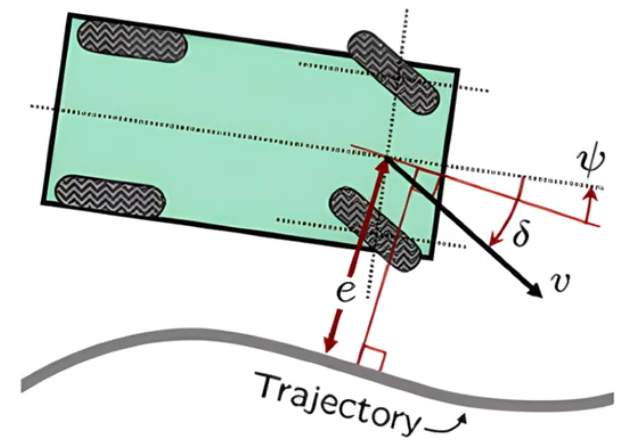
\includegraphics[width=0.85\columnwidth]{Imagens/Controlador Stanley.png}
    \caption{Representação geométrica do controlador Stanley. Fonte: \citet{Hoffmann2007}.}
    \label{fig:controlador_stanley}
\end{figure}

Adotando-se a convenção de que o erro lateral é positivo quando o veículo se encontra à esquerda da trajetória de referência, a lei de controle pode ser expressa por:

\begin{equation}
    \delta =
    \psi -
    \arctan\left(\frac{k e}{v}\right),
    \label{eq:stanley}
\end{equation}

em que $\delta$ representa o ângulo de esterçamento comandado, $k$ é um ganho positivo de controle e $v$ corresponde à velocidade longitudinal do veículo. 

O primeiro termo atua no alinhamento da orientação do veículo com a trajetória, enquanto o segundo corrige o deslocamento lateral. A influência desse último termo diminui com o aumento da velocidade, para um mesmo erro lateral \citep{Hoffmann2007}. 

Em aplicações práticas, a formulação pode incorporar modificações destinadas a melhorar o comportamento do controlador. Entre elas, destaca-se a introdução de um parâmetro de suavização $k_s$ no denominador, que limita a sensibilidade da correção lateral em velocidades próximas de zero \citep{Hoffmann2007}. 

Além disso, pode-se empregar uma ação antecipativa (\textit{feedforward}) baseada na curvatura $\kappa$ da trajetória, utilizando a relação geométrica entre a curvatura e o esterçamento. Essa compensação pode ser expressa por: 

\begin{equation}
    \delta_{ff} =
    k_{ff}\arctan(L_{ff}\kappa),
    \label{eq:stanley_feedforward}
\end{equation}

em que $k_{ff}$ representa o ganho antecipativo e $L_{ff}$ corresponde à distância entre eixos considerada na compensação da curvatura. Também podem ser incorporados termos de amortecimento relacionados à velocidade angular do veículo, com o objetivo de reduzir oscilações do comando de esterçamento \citep{Hoffmann2007}. 

Dessa forma, o método Stanley permite determinar o esterçamento a partir dos desvios geométricos em relação à trajetória, podendo ser complementado por estratégias que considerem a curvatura do percurso e o comportamento da orientação do veículo. 

\subsection{Exemplos de Arquiteturas de Veículos Autônomos}
\label{subsec:arquiteturas_referencia}

O desenvolvimento de veículos autônomos exige a integração de diferentes subsistemas responsáveis por percepção, localização, planejamento e controle. Para organizar essas funções, diferentes plataformas experimentais adotam arquiteturas modulares e distribuídas, permitindo separar responsabilidades, estabelecer mecanismos de comunicação e integrar componentes com diferentes requisitos computacionais.

O veículo Stanley, desenvolvido pela Universidade de Stanford, utilizava uma arquitetura distribuída, organizada em módulos de software responsáveis por funções como percepção do ambiente, localização, planejamento e controle. Essa organização permitia executar diferentes processos de maneira integrada, combinando informações dos sensores com as decisões de navegação e os comandos de atuação do veículo \citep{Thrun2006}.

No Brasil, o projeto CaRINA, desenvolvido pela Universidade de São Paulo (USP), adotou uma arquitetura modular baseada no ROS, permitindo integrar componentes de hardware e software por meio de mecanismos padronizados de comunicação. Essa abordagem favoreceu o desenvolvimento independente dos subsistemas e sua integração em diferentes configurações experimentais \citep{Fernandes2014}.

O veículo IARA, desenvolvido pela Universidade Federal do Espírito Santo (UFES), também apresenta uma arquitetura organizada em subsistemas especializados, abrangendo percepção, localização, tomada de decisão, planejamento de movimento e controle. A integração desses componentes permite transformar as informações obtidas pelos sensores em decisões de navegação e comandos de atuação, possibilitando a operação autônoma do veículo \citep{Badue2021}.
\section{A Plataforma VIDA}
\label{sec:plataforma}

O Veículo Inteligente de Desenvolvimento Aplicado (VIDA) é uma plataforma experimental de pequeno porte, desenvolvida pelo Laboratório de Mobilidade Terrestre (LMT), da Universidade Federal de Lavras (UFLA). Iniciado em 2019, o projeto tem como finalidade disponibilizar um veículo elétrico para o desenvolvimento, a integração e a validação de tecnologias relacionadas à condução autônoma. 

A plataforma foi concebida para apoiar pesquisas nas áreas de instrumentação, localização, navegação e controle de veículos terrestres. Sua utilização permite avaliar algoritmos e sistemas embarcados em condições reais de operação, contribuindo para a aproximação entre o desenvolvimento teórico e a validação experimental. 

A Figura~\ref{fig:vida_atual} apresenta a plataforma VIDA em sua configuração atual, utilizada neste trabalho.

\begin{figure}[htb]
    \centering
    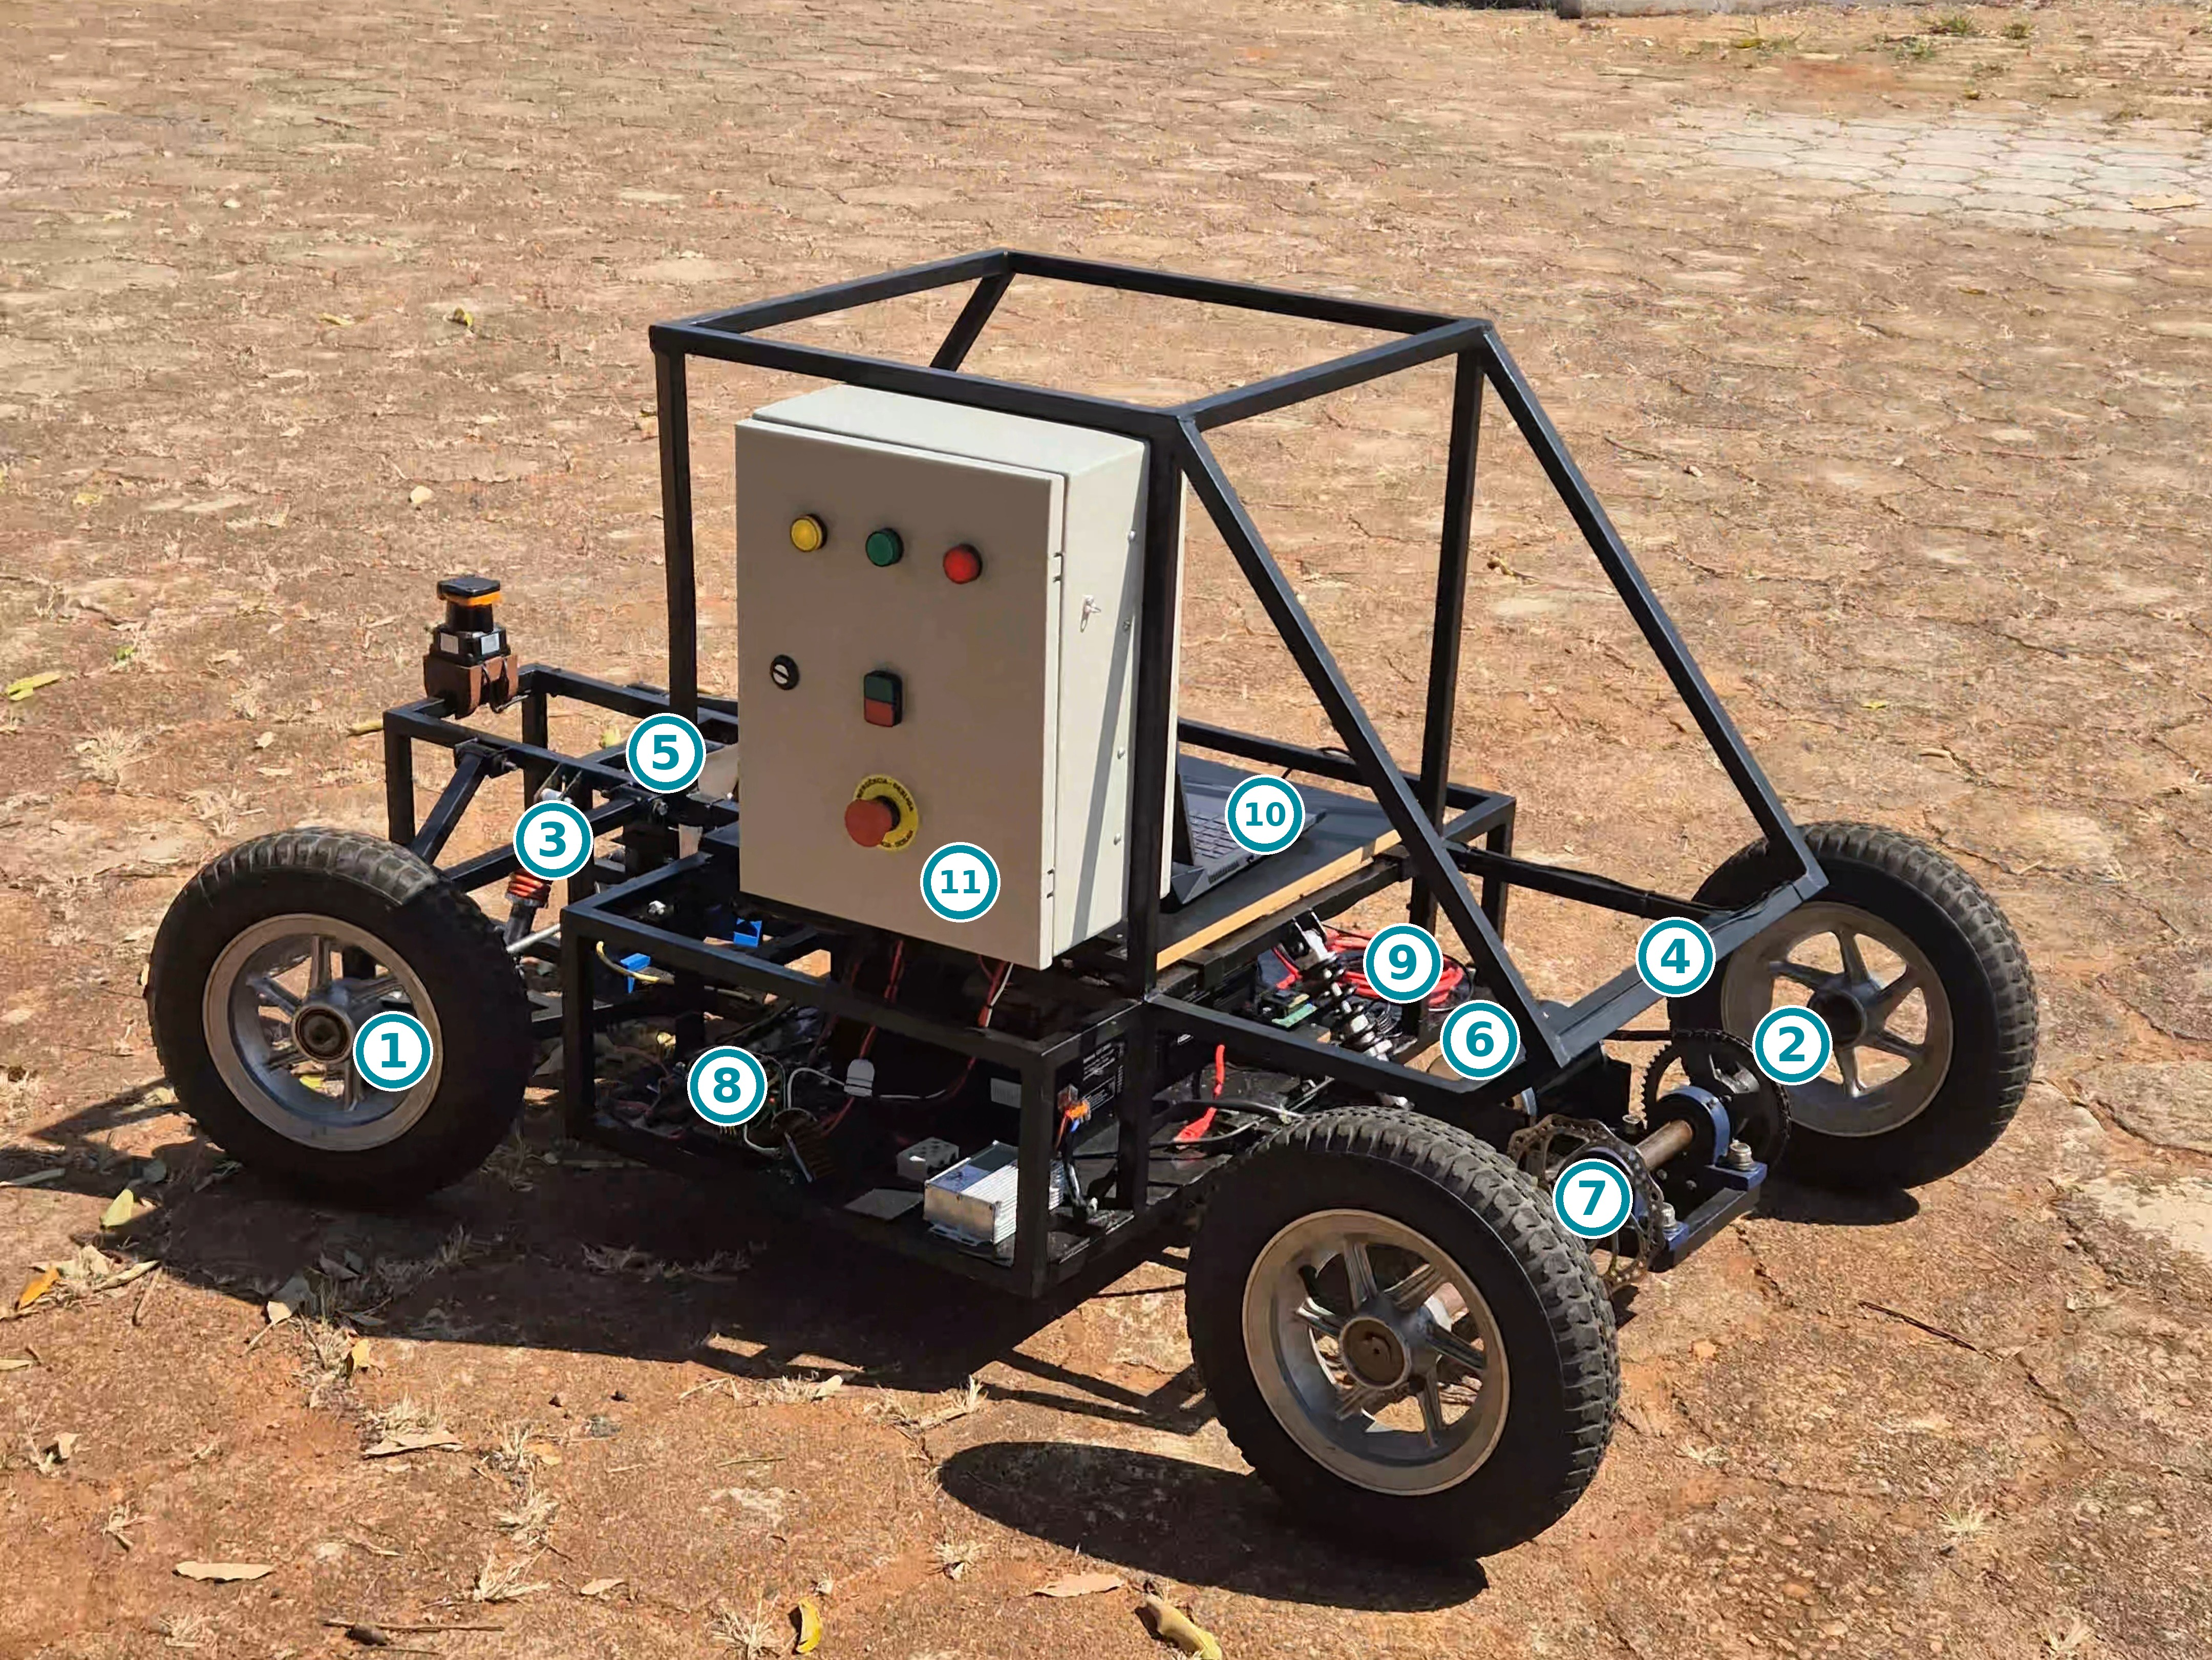
\includegraphics[width=0.72\columnwidth]{Imagens/Vida 1.jpg}
   \caption{Estado atual da plataforma VIDA. Fonte: Acervo do autor.}
    \label{fig:vida_atual}
\end{figure}

\subsection{Estrutura Mecânica}

A estrutura mecânica do VIDA foi desenvolvida em etapas anteriores do projeto, sendo constituída por um chassi metálico modular, com quatro rodas, tração traseira e esterçamento nas rodas dianteiras. Essa configuração permite a instalação de diferentes componentes e instrumentos, conforme as necessidades das pesquisas desenvolvidas na plataforma. 

Durante a evolução do projeto, a estrutura do veículo recebeu modificações, destacando-se a instalação de um suporte metálico elevado, desenvolvido por \citet{Lorenzato2026}. Essa estrutura foi projetada para acomodar câmeras de visão estéreo e permitir o posicionamento do receptor GNSS em relação ao eixo traseiro do veículo.

O sistema de esterçamento também passou por uma modificação, realizada no âmbito das atividades deste trabalho, envolvendo o redimensionamento do motor elétrico e a modificação do conjunto de transmissão mecânica. O novo mecanismo utiliza polias e correia dentada para transmitir o movimento do motor ao sistema de direção, conforme apresentado na Figura~\ref{fig:estercamento_vida}.

\begin{figure}[htb]
    \centering
    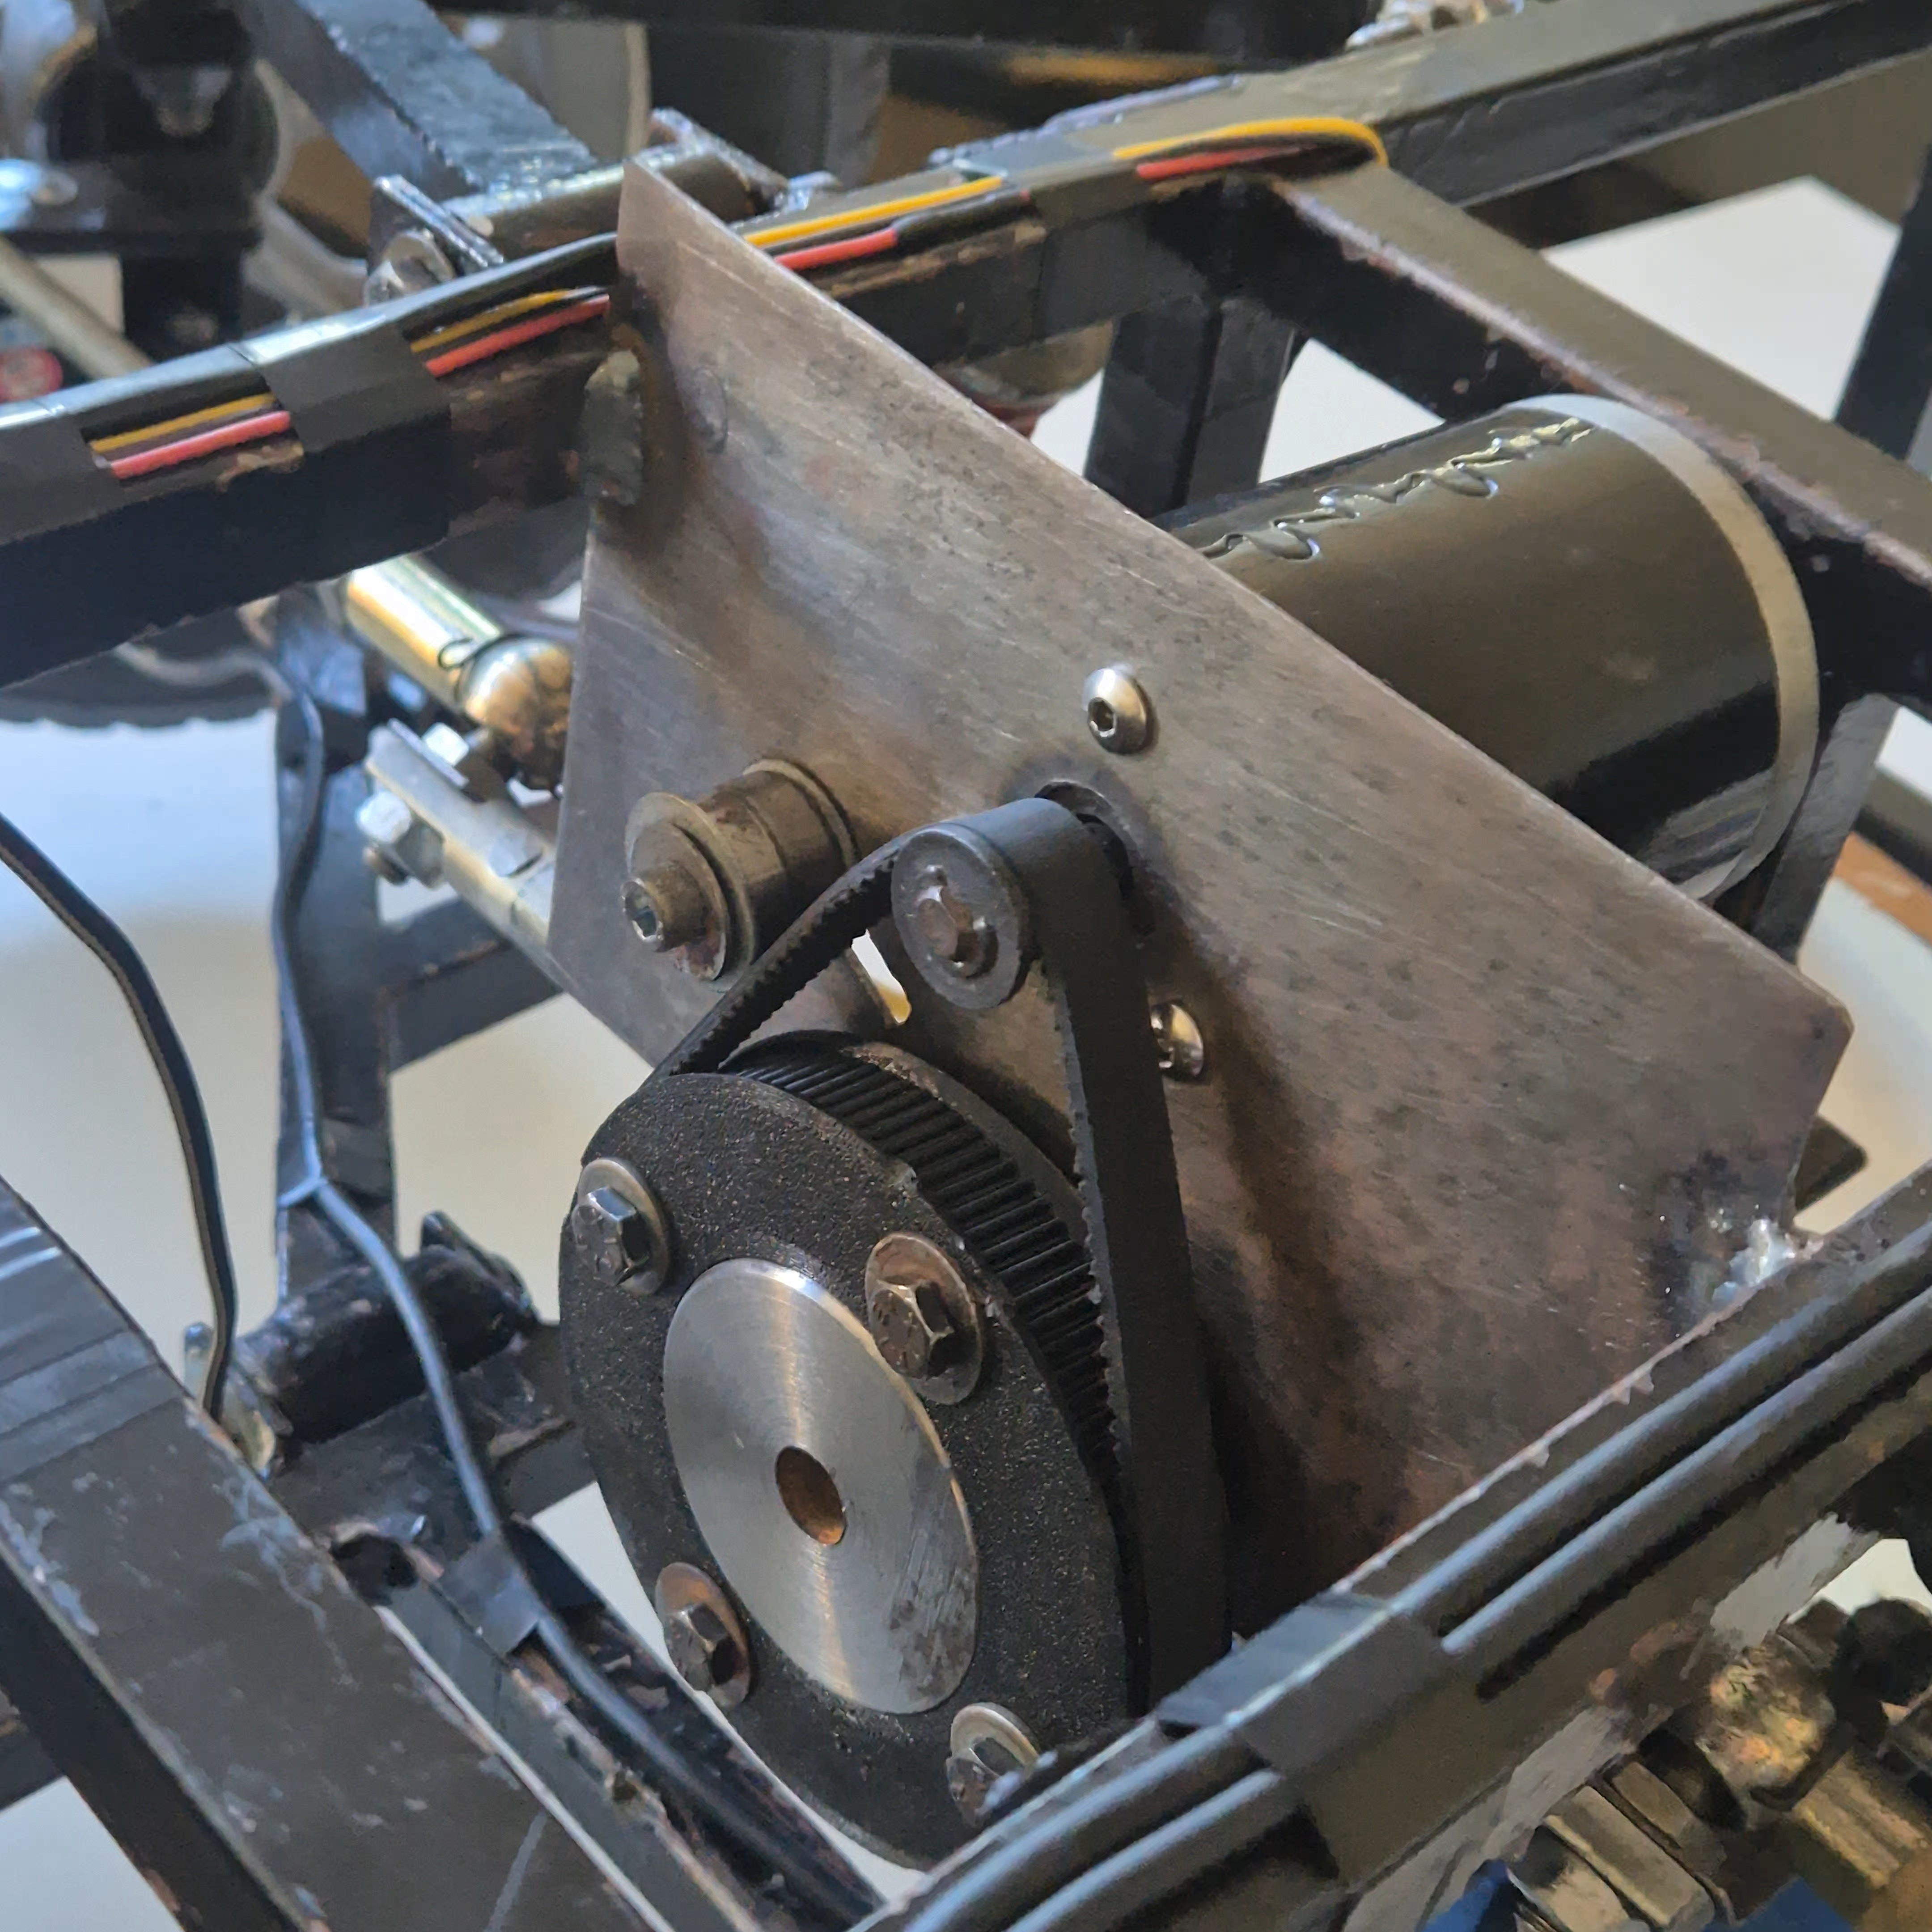
\includegraphics[width=0.72\columnwidth]{Imagens/Conjunto de esterçamento.jpg}
   \caption{Conjunto de esterçamento
    do VIDA. Fonte: Acervo do autor.}
    \label{fig:estercamento_vida}
\end{figure}


\subsection{Sistema Elétrico}

O sistema elétrico do VIDA passou por uma reformulação para atender às necessidades de alimentação, acionamento e integração dos componentes embarcados. A arquitetura implementada utiliza quatro baterias de 12 V, sendo três conectadas em série para formar um banco de 36 V, destinado aos circuitos de potência, e uma bateria independente de 12 V, responsável pela alimentação dos sistemas eletrônicos e periféricos.

A distribuição de energia foi organizada em um painel elétrico centralizado, que reúne os dispositivos de proteção, os conversores de tensão e os circuitos de comando. Os bancos de alimentação possuem entradas distintas no painel, buscando reduzir a interferência dos acionamentos de potência sobre os circuitos eletrônicos. O esquema elétrico completo do sistema de alimentação e distribuição de energia é apresentado no Apêndice~\ref{ap:esquema_eletrico}.

No circuito auxiliar, a tensão proveniente da bateria de 12 V é inicialmente elevada para 18 V por meio de um conversor CC-CC. Essa tensão é utilizada diretamente na alimentação do sensor LVDT e como entrada de um segundo estágio de regulação, responsável por fornecer uma tensão estabilizada de 12 V aos dispositivos periféricos. A partir dessa saída, um terceiro conversor reduz a tensão para 5 V, utilizada na alimentação dos componentes que operam nesse nível de tensão.

O circuito principal de 36 V alimenta os sistemas de potência e de comando. Parte dessa alimentação é convertida para 12 V, destinada aos dispositivos de operação, sinalização e acionamento dos relés auxiliares. O barramento de potência é interrompido por um relé principal normalmente aberto, cuja saída fornece 36 V ao sistema de tração e alimenta um conversor CC-CC, responsável por fornecer 24 V ao motor de esterçamento.

O painel dispõe de chave seccionadora geral, disjuntores de proteção, botões de acionamento, dispositivo de parada de emergência e sinalizadores luminosos. A lógica de comando utiliza relés auxiliares para controlar a habilitação do barramento de potência e disponibilizar um sinal lógico de 5 V aos sistemas de controle quando o veículo está habilitado.

A Figura~\ref{fig:painel_eletrico_vida} apresenta a implementação física do painel, destacando a organização dos conversores, dispositivos de proteção, relés e bornes de distribuição, bem como os elementos de comando instalados na porta. 

\begin{figure}[htb]
    \centering
    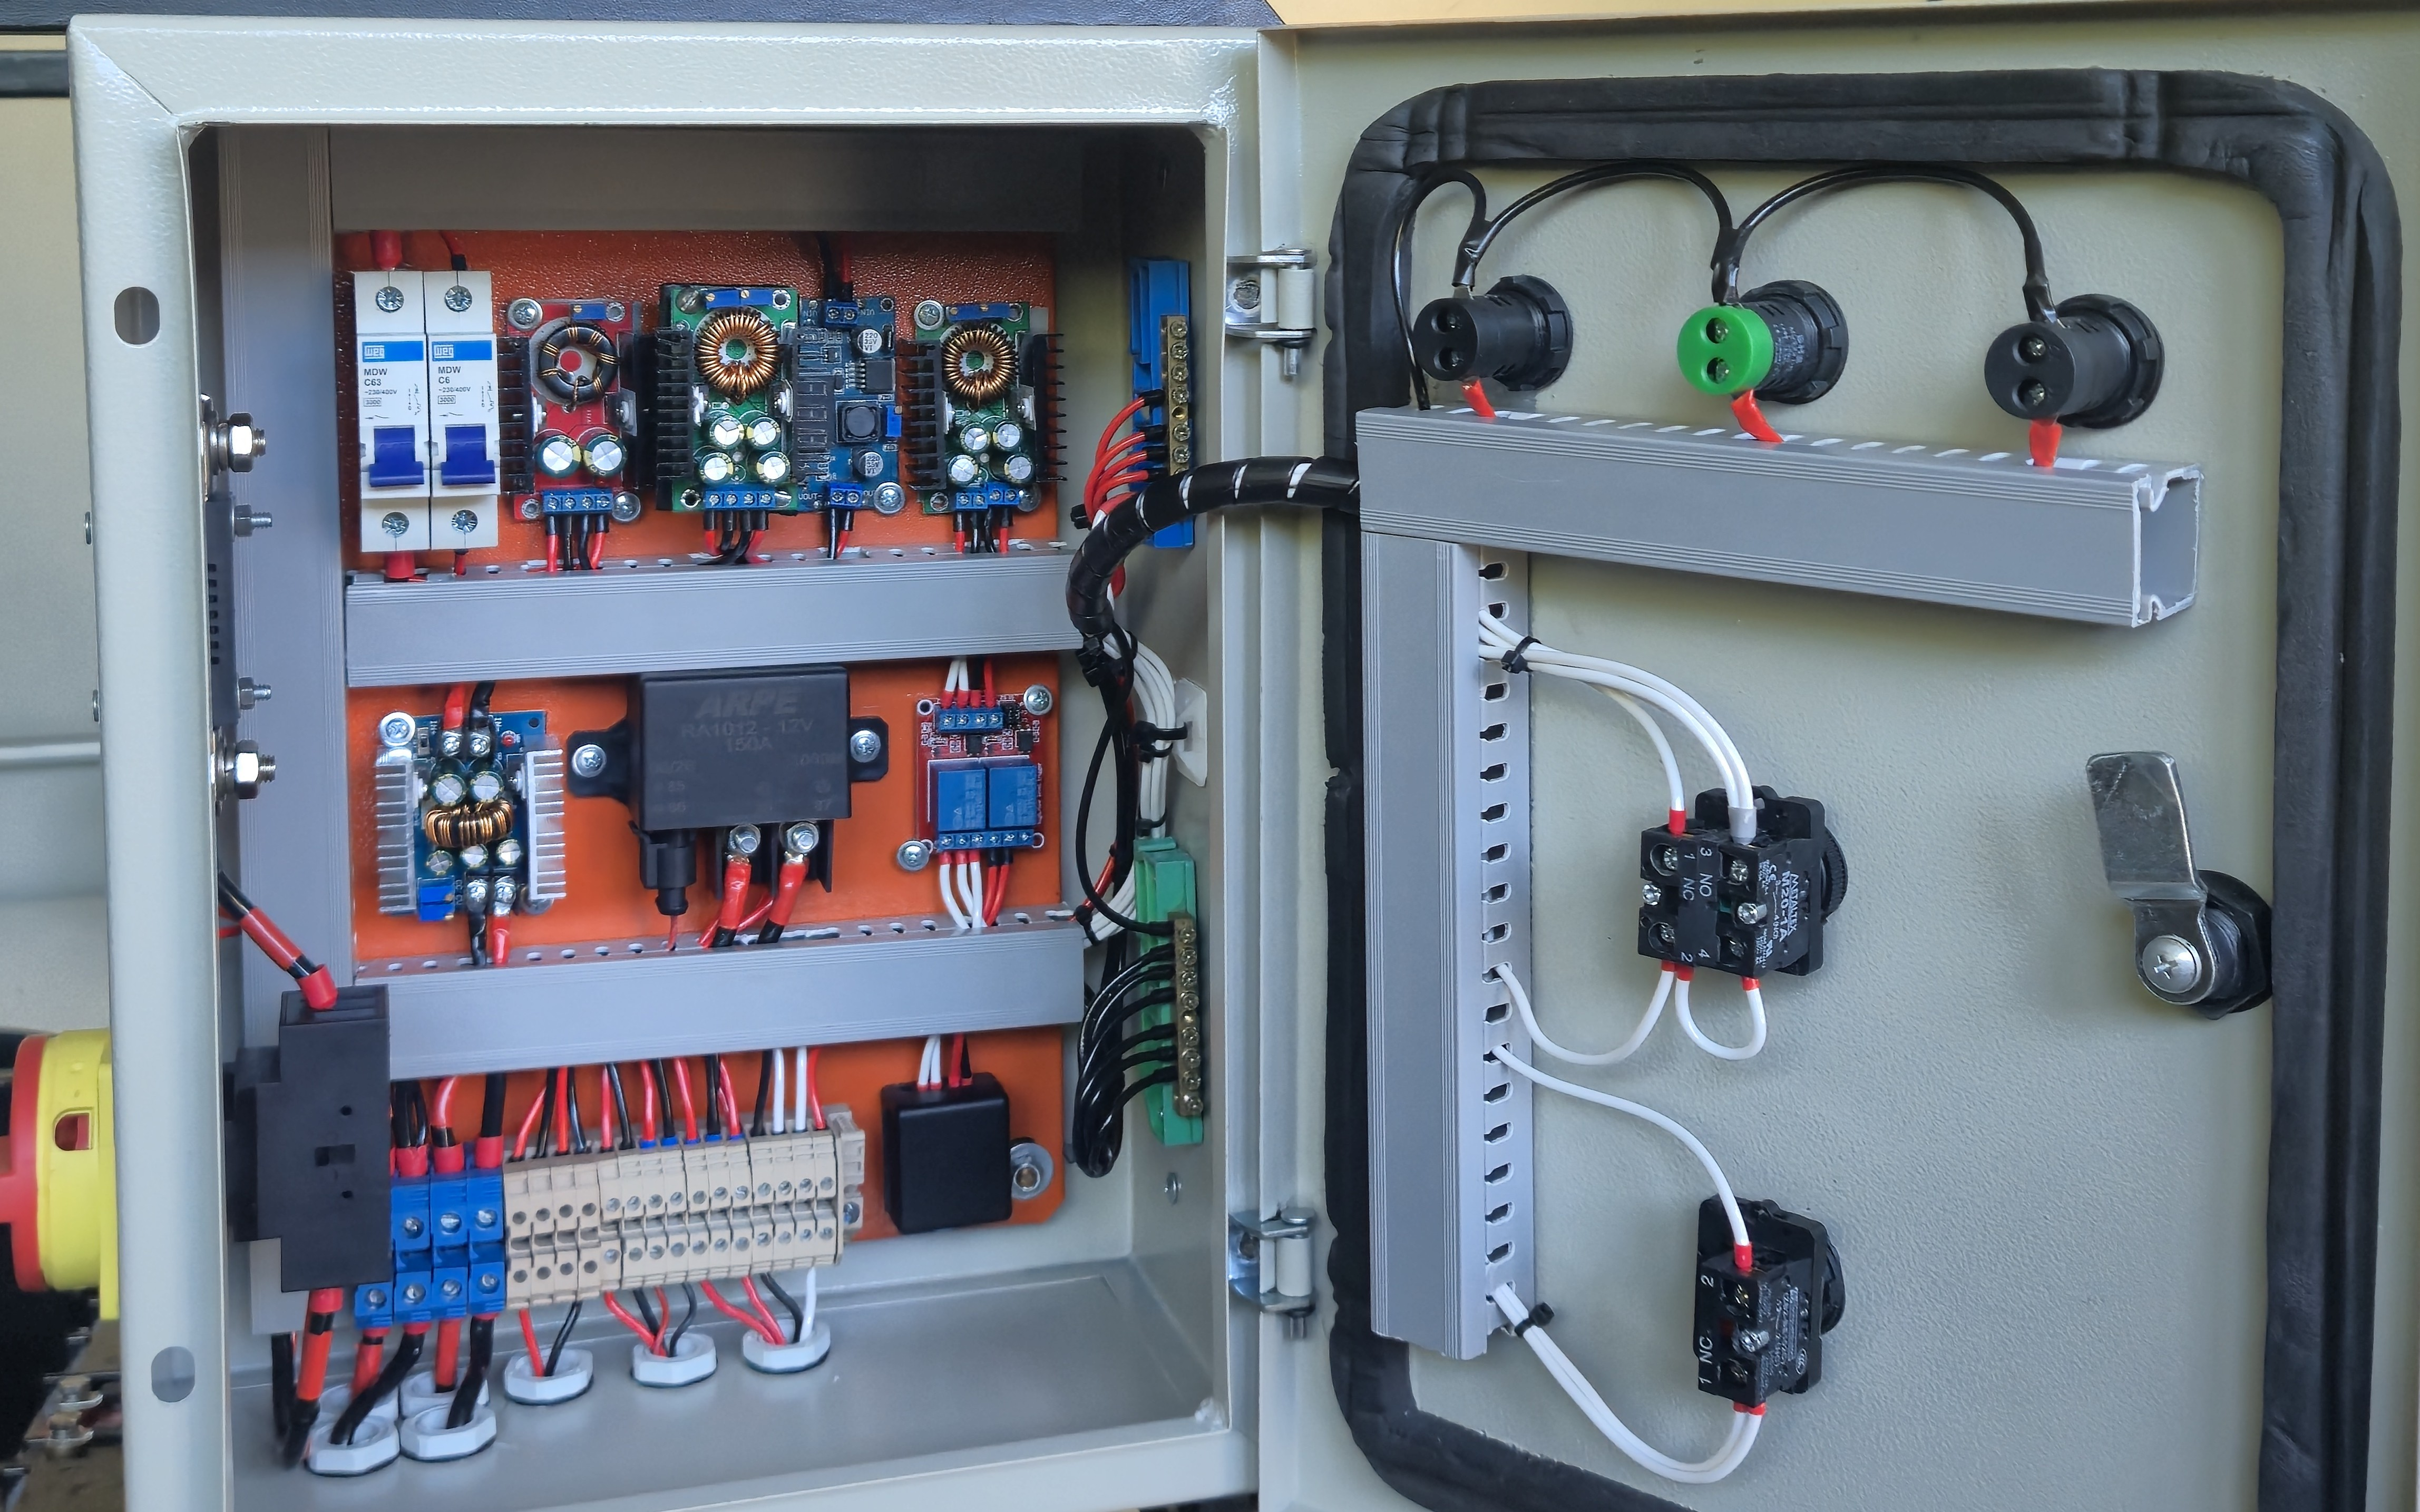
\includegraphics[width=0.85\columnwidth]{Imagens/Painel.jpg}
    \caption{Vista interna do painel elétrico do VIDA. Fonte: Acervo do autor.}
    \label{fig:painel_eletrico_vida}
\end{figure}


\subsection{Instrumentação e Sensoriamento}

A instrumentação do VIDA é composta por sensores destinados à aquisição de informações relacionadas ao movimento, à orientação e à localização do veículo. Para o desenvolvimento deste trabalho, foram utilizados três encoders incrementais, um sensor de deslocamento linear LVDT e um receptor GNSS com sensores inerciais integrados.

Os encoders incrementais são responsáveis pela medição da rotação das rodas, permitindo estimar o deslocamento e a velocidade longitudinal do veículo. Dois sensores estão instalados nas rodas dianteiras, enquanto o terceiro está instalado no eixo traseiro. Todos possuem dois canais de saída em quadratura, permitindo a identificação do sentido de rotação. A aquisição utiliza decodificação em quadratura completa, com resoluções configuradas de 720 contagens por revolução para os encoders dianteiros e 1440 para o traseiro.

O sensor LVDT (\textit{Linear Variable Differential Transformer}) é utilizado para medir o deslocamento linear do mecanismo de direção. Por meio de uma relação de calibração, essa medição permite determinar o ângulo de esterçamento das rodas dianteiras, fornecendo a realimentação necessária ao sistema de controle de direção.

Para o posicionamento global, utiliza-se o receptor GNSS u-blox ZED-F9R, que permite o emprego de correções RTK para obtenção de estimativas de posição de maior precisão. O dispositivo também integra sensores inerciais, incluindo um giroscópio, cujas informações de velocidade angular contribuem para a estimação da orientação do veículo.

A Tabela~\ref{tab:sensores_vida} apresenta um resumo dos principais sensores utilizados na plataforma.

\begin{table}[htb]
    \centering
    \caption{Instrumentação utilizada na plataforma VIDA.}
    \label{tab:sensores_vida}
    \small
    \begin{tabular}{lll}
        \hline
        \textbf{Dispositivo} &
        \textbf{Qtd.} &
        \textbf{Grandeza medida} \\
        \hline
        Encoder dianteiro & 2 & Rotação das rodas dianteiras \\
        Encoder traseiro & 1 & Rotação do eixo traseiro \\
        LVDT & 1 & Angulo de esterçamento \\
        GNSS ZED-F9R & 1 & Posição geográfica \\
        Giroscópio ZED-F9R & 1 & Velocidade angular \\
        \hline
    \end{tabular}
\end{table}
\section{Arquitetura Computacional}
\label{sec:arquitetura}

A arquitetura computacional do VIDA foi desenvolvida de forma distribuída e modular, sendo composta por três níveis de processamento: um microcontrolador ESP32, um computador embarcado Odroid e um notebook. Essa organização distribui as funções de aquisição, controle, localização e navegação entre dispositivos com capacidades computacionais distintas e estabelece uma infraestrutura escalável e capaz de receber novos subsistemas. Embora os algoritmos atualmente implementados sejam computacionalmente leves, a manutenção de um nível adicional de processamento permite validar a comunicação entre dispositivos e prepara a plataforma para aplicações futuras mais exigentes, como percepção visual, planejamento de movimento e inteligência artificial.

\subsection{Comunicação e Integração dos Subsistemas}

A integração dos três níveis de processamento é realizada por meio do ROS~2 Humble, cuja arquitetura se basea em nós, tópicos e serviços e permite a comunicação entre componentes distribuídos \citep{Macenski2022}. A Figura~\ref{fig:arquitetura_computacional} apresenta a organização geral da arquitetura e as principais interfaces de comunicação entre os dispositivos.

\begin{figure}[htb]
    \centering
    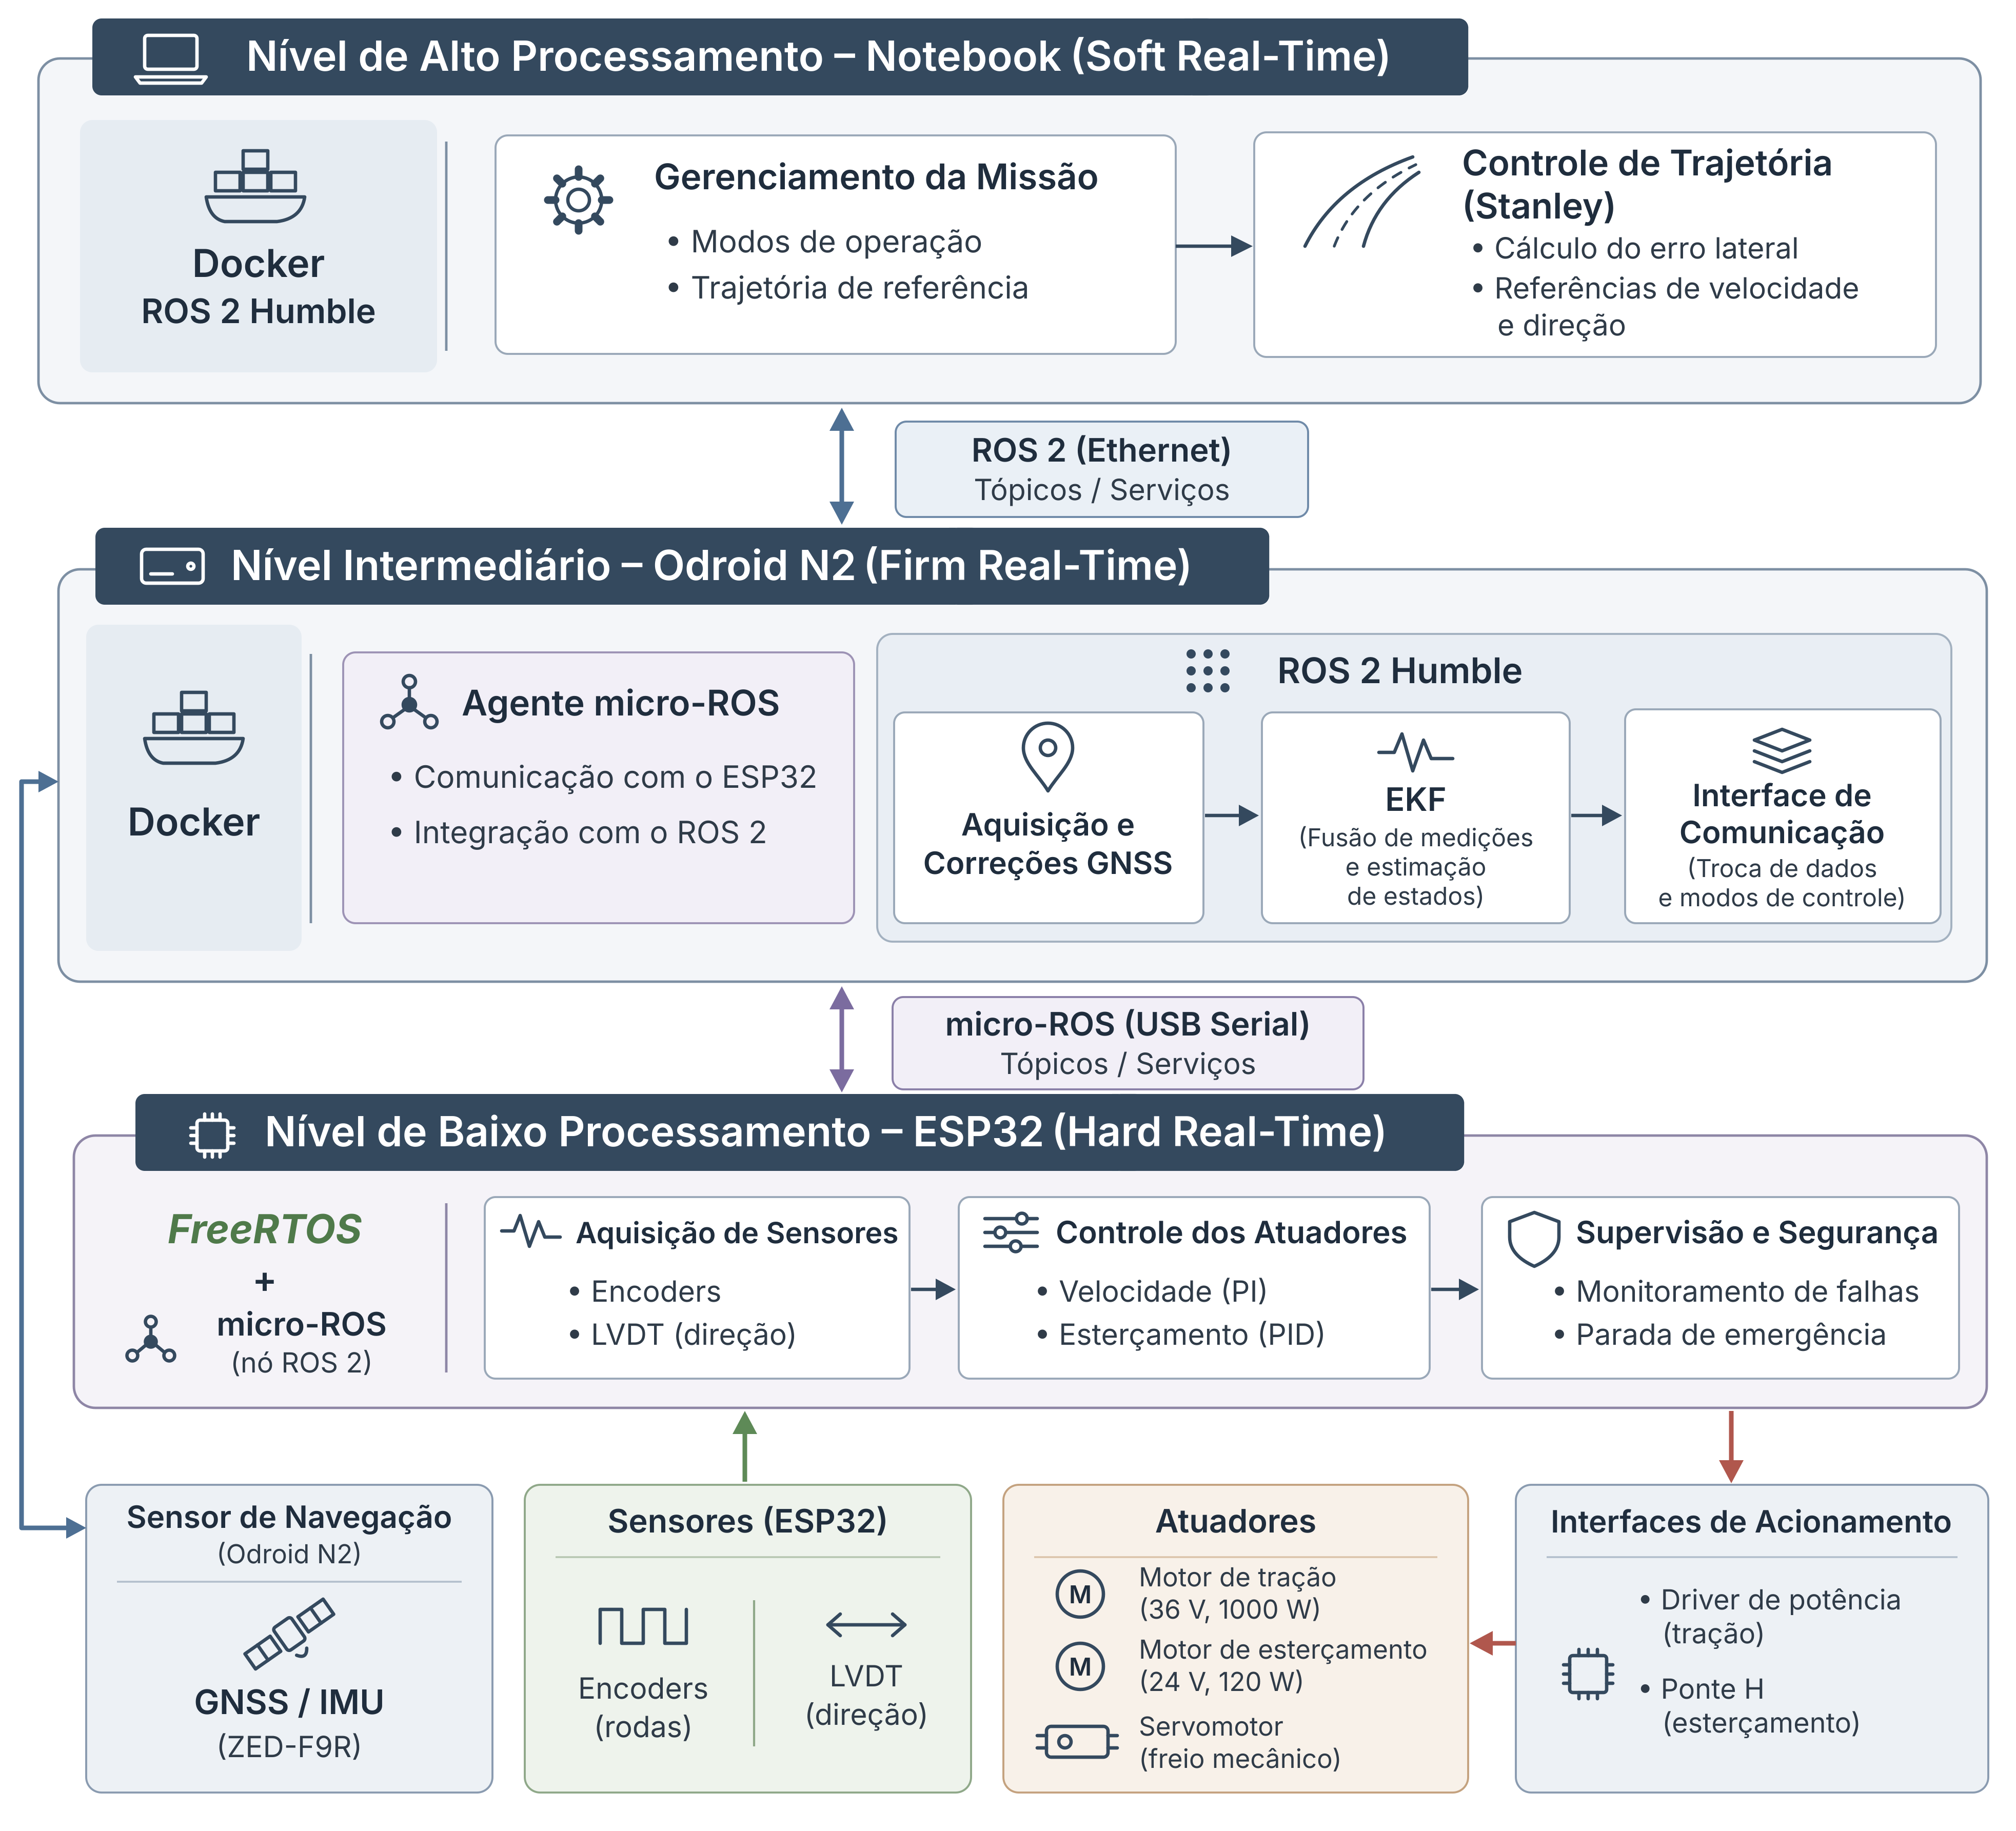
\includegraphics[width=\columnwidth]{Imagens/Arquitetura computacional.png}
    \caption{Arquitetura computacional plataforma VIDA. Fonte: Elaborado pelo autor.}
    \label{fig:arquitetura_computacional}
\end{figure}

A comunicação entre o ESP32 e a Odroid é realizada por uma conexão serial USB a 921\,600~bit/s, utilizando o micro-ROS e o protocolo XRCE-DDS. O agente micro-ROS executado na Odroid estabelece a ponte entre o microcontrolador e a rede DDS do ROS~2.

A Odroid e o notebook são conectados por um cabo Ethernet ponto a ponto, com endereçamento IP fixo. Por essa conexão trafegam as mensagens DDS entre os nós ROS~2 dos dois dispositivos, incluindo os estados estimados, as informações de navegação e as referências de controle. Ambos utilizam a implementação Fast DDS, configurada para transporte exclusivamente por UDP, no mesmo domínio ROS~2.

Adicionalmente, o notebook compartilha com a Odroid, por tradução de endereços de rede (NAT), a conexão com a Internet obtida por rede sem fio. Esse compartilhamento fornece o acesso necessário para que o cliente NTRIP receba as correções RTK.

A utilização de containers Docker na Odroid e no notebook padroniza os ambientes de execução, encapsulando as dependências dos componentes ROS~2 e reduzindo problemas de compatibilidade com os sistemas hospedeiros.

Dessa forma, a arquitetura implementada estabelece uma infraestrutura modular para aquisição, controle, localização e navegação, permitindo a comunicação entre componentes executados em diferentes unidades de processamento e preservando a possibilidade de redistribuição e expansão das funções computacionais da plataforma.

\subsection{Nível de Baixo Processamento -- ESP32}

O nível de baixo processamento é constituído por um microcontrolador ESP32, responsável pela aquisição dos sensores de velocidade e esterçamento, execução dos controladores de baixo nível, geração dos sinais de acionamento e pela supervisão das condições de segurança. O firmware utiliza o sistema operacional de tempo real FreeRTOS \citep{Barry2024FreeRTOS}, que organiza essas funções em tarefas periódicas distribuídas entre os dois núcleos do processador: o núcleo 1 é dedicado às tarefas de tempo real (aquisição, segurança e controle), enquanto o núcleo 0 concentra a comunicação e a supervisão das demais tarefas.

A aquisição dos dados compreende a leitura dos três encoders incrementais, e do sensor LVDT. A partir dessas medições, o firmware determina o ângulo de esterçamento e sua taxa de variação, bem como as velocidades e acelerações das rodas. Como as tarefas são executadas concorrentemente nos dois núcleos, as medições e as referências recebidas são compartilhadas por meio de \textit{snapshots}, que são cópias completas gravadas e lidas em seções críticas protegidas pelo mecanismo do FreeRTOS \textit{spinlock} (\texttt{portMUX}). Assim, cada tarefa obtém um conjunto coerente de dados, sem valores parcialmente atualizados e sem bloquear as tarefas de tempo real.

O controle dos atuadores é realizado por duas malhas independentes, um controlador PI regula a velocidade longitudinal, realimentado pela média das velocidades das rodas dianteiras, e um controlador PID regula o ângulo de esterçamento, realimentado pelo LVDT. As referências utilizadas por essas malhas são recebidas por meio do micro-ROS. Os comandos resultantes são encaminhados aos motores de esterçamento, tração,  e servomotor do freio por um único módulo de acionamento, que concentra o acesso aos atuadores. A implementação dos controladores e seus parâmetros são detalhados na Seção~\ref{sec:baixo_nivel}.

Embora os algoritmos de controle sejam executados localmente, a liberação do movimento depende de um conjunto de condições verificadas por uma tarefa de segurança de maior prioridade. O movimento somente é permitido quando o enable físico está acionado, a habilitação lógica foi recebida há menos de 1,5~s, as referências de velocidade e de esterçamento foram atualizadas há menos de 200~ms, os sensores estão válidos e não há indícios de falha, como esterçamento travado ou em sentido oposto ao comandado. Caso qualquer condição deixe de ser satisfeita, os comandos dos motores são anulados e o freio é aplicado progressivamente até a frenagem total. De forma complementar, uma rotina de supervisão executada no núcleo 0 a cada 10~ms monitora a atividade das tarefas do núcleo 1 e desativa os atuadores caso alguma delas permaneça mais de 50~ms sem executar.

A Figura~\ref{fig:arquitetura_tasks_esp32} apresenta a organização das tarefas executadas no ESP32, seus períodos de execução e o fluxo de processamento de cada uma.

\begin{figure}[htb]
    \centering
    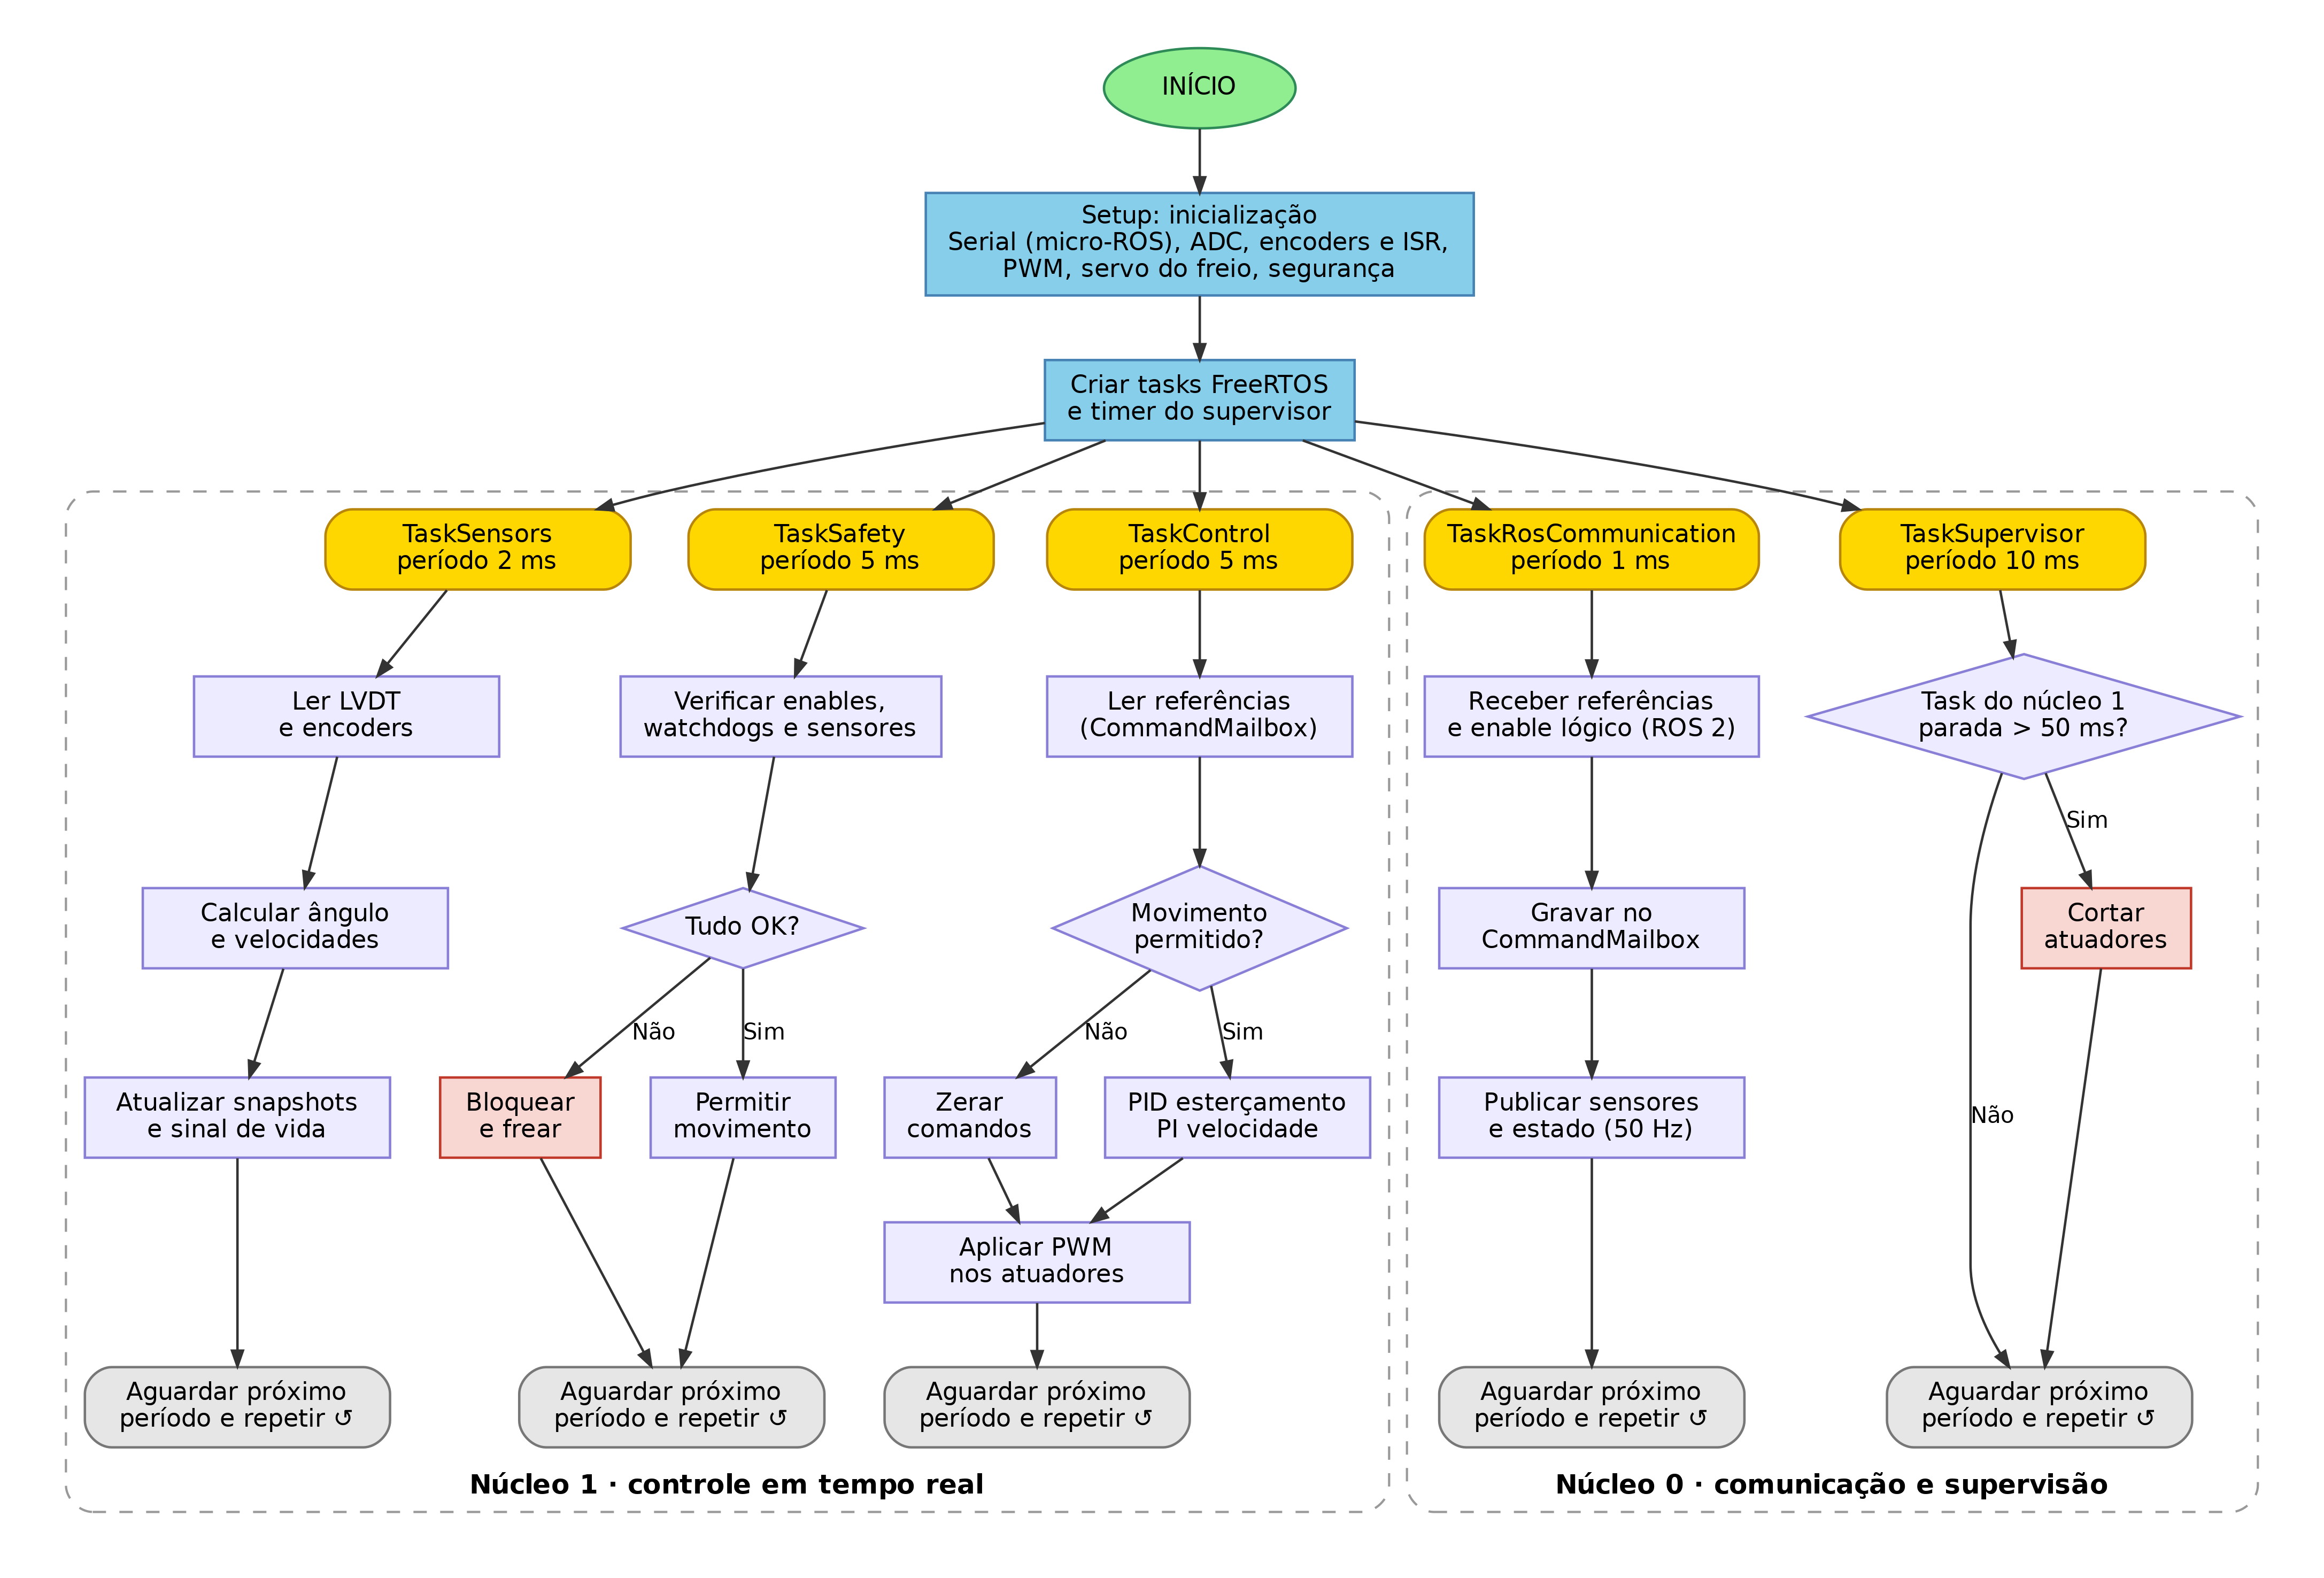
\includegraphics[width=\columnwidth]{Imagens/fluxograma_esp32.png}
    \caption{Diagrama das tarefas FreeRTOS no ESP32. Fonte: Elaborado pelo autor.}
    \label{fig:arquitetura_tasks_esp32}
\end{figure}

\subsection{Nível Intermediário -- Odroid N2}

O nível intermediário de processamento é constituído por um computador embarcado Odroid N2 com sistema operacional Linux, responsável pela integração do microcontrolador à infraestrutura ROS~2 e pela execução dos componentes de localização e estimação de estados do veículo.

Os ambientes de execução são organizados em dois containers Docker. O primeiro é dedicado ao agente micro-ROS, que estabelece a comunicação com o ESP32 e disponibiliza suas mensagens aos demais nós. O segundo reúne os nós executados no ROS~2 Humble: o driver do receptor GNSS, o cliente NTRIP, o estimador de estados e o nó de habilitação lógica.

O receptor GNSS u-blox ZED-F9R está conectado à Odroid por USB e fornece posições geográficas e medições da unidade inercial integrada. O cliente NTRIP, executado como um nó ROS~2, obtém as correções RTK de uma rede pública de estações de referência e as encaminha ao receptor pela mesma conexão USB, permitindo o posicionamento com precisão centimétrica. As posições GNSS são fundidas aos demais dados por meio de um filtro de Kalman estendido (EKF). A implementação do EKF é detalhada na Seção~\ref{sec:estimacao}.

A Odroid também executa o nó responsável por gerar o sinal de habilitação lógica enviado ao ESP32. Esse sinal permanece ativo enquanto o notebook recebe mensagens do controle de operação manual. A perda de comunicação com o operador, portanto, leva o ESP32 a bloquear o movimento e aplicar o freio.

A separação dos ambientes em containers isola as dependências do agente micro-ROS e dos demais componentes ROS~2, reduzindo conflitos de configuração efacilitando a manutenção e a atualização dos diferentes módulos.

\subsection{Nível de Alto Processamento -- Notebook}

O nível de alto processamento é executado em um notebook, responsável pelas funções de navegação, gerenciamento dos modos de operação e interação com o operador. Seus componentes de software são executados em ROS~2 Humble, organizado em container Docker, mantendo a compatibilidade com os demais dispositivos da arquitetura.

O sistema de navegação utiliza as estimativas do EKF para realizar o acompanhamento de uma trajetória previamente gravada com RTK. O controlador Stanley, é executado a cada nova estimativa de estado e sua implementação é detalhada na Seção~\ref{sec:seguimento_trajetoria}.

O notebook também executa o gerenciador de modos de operação, responsável por coordenar as transições entre a condução manual e a navegação autônoma, supervisionar as condições operacionais do veículo e encaminhar as referências de controle ao ESP32. O funcionamento desse gerenciador é detalhado na Seção~\ref{subsec:gerenciamento_navegacao}.

Para a condução manual, o operador utiliza um gamepad conectado ao notebook, cujos comandos são convertidos em referências de velocidade e de esterçamento e transmitidos pela mesma infraestrutura de comunicação utilizada no modo autônomo. Além disso, o notebook disponibiliza ferramentas para gravação e validação de trajetórias de referência e um painel de supervisão para o monitoramento do veículo.

A concentração dessas funções no notebook mantém os componentes de alto nível independentes das tarefas de aquisição e controle executadas nos demais dispositivos, facilitando a incorporação futura de algoritmos mais exigentes computacionalmente.



\section{Controle de Baixo Nível}
\label{sec:baixo_nivel}

O controle de baixo nível do VIDA tem como objetivo garantir o acompanhamento das referências de velocidade longitudinal e ângulo de esterçamento estabelecidas pelo sistema de navegação ou pela operação manual. Para isso, são empregadas duas malhas de controle, responsáveis por compensar os desvios entre as referências solicitadas e as grandezas medidas pelos sensores embarcados. As ações de controle resultantes são convertidas em comandos para os sistemas de tração, esterçamento e frenagem, respeitando as limitações operacionais e os mecanismos de segurança da plataforma. As estratégias de controle e suas respectivas implementações são apresentadas nas subseções seguintes.

\subsection{Controle de Esterçamento}
\label{subsec:controle_esterçamento}

O controle de esterçamento tem como finalidade regular o ângulo das rodas dianteiras a partir de uma referência estabelecida pelo sistema de navegação ou pela operação manual. Para isso, foi implementado um controlador proporcional-integral-derivativo (PID) discreto, executado a uma frequência nominal de 200~Hz. A realimentação é fornecida pelo sensor LVDT, cuja medição de deslocamento linear é convertida em ângulo de esterçamento por meio de uma relação de calibração.

A lei de controle pode ser expressa por:

\begin{equation}
u_{\delta}(t) =
K_p e_{\delta}(t)
+ K_i \int_0^t e_{\delta}(\tau)\,d\tau
- K_d \dot{\delta}_{m,f}(t)
\end{equation}

em que $u_{\delta}$ representa o sinal de controle, $K_p$, $K_i$ e $K_d$ são os ganhos proporcional, integral e derivativo, respectivamente, e $e_{\delta}$ corresponde à diferença entre o ângulo de referência e o ângulo medido. O termo $\dot{\delta}_{m,f}$ representa a taxa de variação filtrada do ângulo de esterçamento medido.

Uma particularidade dessa implementação é a aplicação da ação derivativa sobre a medição, em vez de diretamente sobre o erro de controle. Essa estratégia evita que alterações abruptas da referência produzam picos na parcela derivativa, fenômeno conhecido como \textit{derivative kick}, contribuindo para uma resposta mais suave do sistema de acionamento \citep{AstromHagglund2006}. 

Antes de ser utilizada pela malha de controle, a referência de esterçamento é submetida a restrições de amplitude e de taxa de variação. O ângulo solicitado é limitado à faixa de $\pm20^\circ$, enquanto sua variação máxima é estabelecida em $40^\circ/\mathrm{s}$. Essas restrições reduzem solicitações bruscas ao mecanismo de direção e contribuem para manter o comando dentro da faixa operacional definida para o veículo.

Além das ações PID, o controlador incorpora recursos destinados a melhorar o comportamento do sistema diante das características do acionamento eletromecânico. Entre eles estão uma zona morta com histerese, a compensação do atrito estático e mecanismos de integração condicionada e anti-windup. A zona morta com histerese contribui para evitar acionamentos sucessivos próximos à condição de equilíbrio, enquanto a compensação do atrito estático auxilia no início do movimento do mecanismo. Os mecanismos associados à ação integral, por sua vez, limitam seu acúmulo em condições nas quais o esforço de controle não pode ser integralmente aplicado.

O firmware também considera restrições associadas aos limites físicos de esterçamento. Embora a referência de operação seja limitada a $\pm20^\circ$, o mecanismo possui um limite de segurança de $\pm25^\circ$. Dessa forma, são impedidos comandos que possam ampliar o esterçamento quando o ângulo medido já se encontra além da faixa permitida.

A Figura~\ref{fig:controle_esterçamento} apresenta a estrutura da malha fechada de controle de esterçamento, reunindo os elementos descritos anteriormente. O diagrama destaca o processamento da referência, a atuação do controlador PID, os mecanismos de compensação e limitação dos comandos, o acionamento do motor de direção e a realimentação fornecida pelo sensor LVDT.

% -----------------------------------------------------------
% FIGURA: DIAGRAMA DA MALHA FECHADA DE ESTERÇAMENTO
% Manter o caminho da imagem já utilizado no seu projeto.
% -----------------------------------------------------------
\begin{figure}[htb]
    \centering
    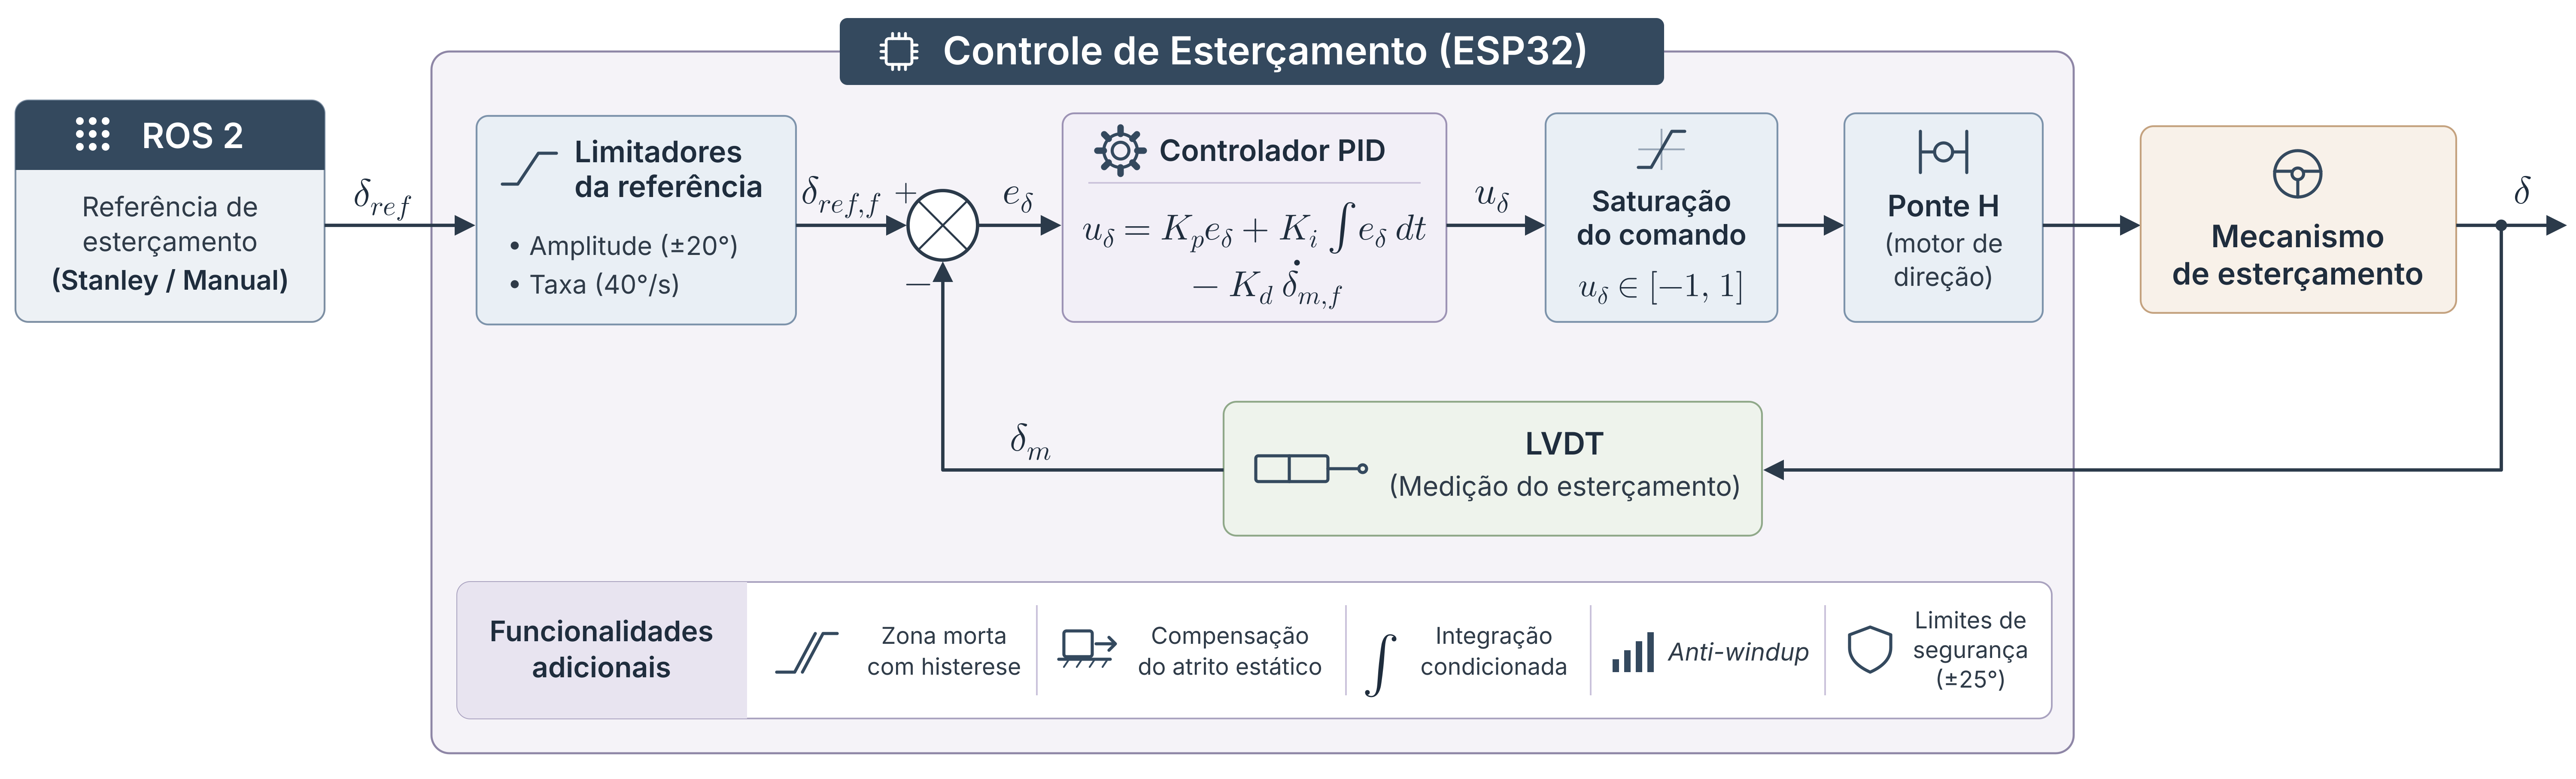
\includegraphics[width=\columnwidth]{Imagens/Malha de controle esterçamento.png}
    \caption{Diagrama da malha fechada de controle do ângulo de esterçamento. Fonte: Elaborado pelo autor.}
    \label{fig:controle_esterçamento}
\end{figure}

Os ganhos do controlador foram inicialmente ajustados com o auxílio de simulações e posteriormente refinados por meio de ensaios experimentais na plataforma VIDA. A Tabela~\ref{tab:parametros_esterçamento} apresenta os ganhos e os limites operacionais adotados na configuração utilizada durante a validação experimental.

\begin{table}[htb]
    \centering
    \caption{Parâmetros do controlador de esterçamento.}
    \label{tab:parametros_esterçamento}
    \begin{tabular}{lc}
        \hline
        \textbf{Parâmetro} & \textbf{Valor} \\
        \hline
        Ganho proporcional ($K_p$) & 0,05 \\
        Ganho integral ($K_i$) & 0,10 \\
        Ganho derivativo ($K_d$) & 0,002 \\
        Limite da referência & $\pm20^\circ$ \\
        Limite de segurança & $\pm25^\circ$ \\
        Taxa máxima da referência & $40^\circ/\mathrm{s}$ \\
        Frequência de controle & 200~Hz \\
        \hline
    \end{tabular}
\end{table}

\subsection{Controle de Velocidade Longitudinal}
\label{subsec:controle_velocidade}

Para regular a velocidade longitudinal do VIDA, foi adotada uma estratégia de controle em malha fechada baseada em um controlador proporcional-integral (PI) discreto, executado a uma frequência nominal de 200~Hz. O controlador determina o esforço necessário para acompanhar a velocidade de referência, utilizando as medições dos encoders como realimentação. A ação de controle resultante é utilizada para coordenar os sistemas de tração e frenagem, permitindo tanto a aceleração quanto a desaceleração do veículo.

A realimentação utiliza a média das velocidades medidas pelos encoders instalados nas rodas dianteiras, que não são diretamente acionadas pelo sistema de tração. Essa configuração reduz a influência de eventuais perdas de aderência da roda traseira motriz sobre a medição da velocidade longitudinal. A velocidade utilizada pelo controlador é calculada por:

\begin{equation}
v_m = \frac{v_{de} + v_{dd}}{2}
\end{equation}

em que $v_m$ representa a velocidade longitudinal medida, enquanto $v_{de}$ e $v_{dd}$ correspondem às velocidades medidas nas rodas dianteiras esquerda e direita, respectivamente. 

A partir da velocidade medida, o controlador determina o erro em relação à referência recebida e calcula o esforço necessário para sua correção. A lei de controle PI pode ser expressa por:

\begin{equation}
u_v(t) = K_p e_v(t) + K_i \int_0^t e_v(\tau)\,d\tau
\end{equation}

em que $u_v$ representa o esforço de controle longitudinal normalizado, $K_p$ e $K_i$ são os ganhos proporcional e integral, respectivamente, e $e_v$ corresponde à diferença entre a velocidade de referência e a velocidade medida. Valores positivos de $u_v$ são utilizados para gerar comandos de tração, enquanto valores negativos são tratados pela lógica de desaceleração e frenagem.

Antes de ser aplicada ao controlador, a referência de velocidade é submetida a restrições de amplitude e de taxa de variação. A velocidade máxima permitida é de $2,5~\mathrm{m/s}$, enquanto rampas de aceleração e desaceleração estabelecem transições graduais entre diferentes condições de movimento. A aceleração padrão é definida em $0,4~\mathrm{m/s^2}$, podendo ser alterada se encaminhada pelo ROS2 junto com a referência de velociade. A desaceleração máxima é limitada a $1,0~\mathrm{m/s^2}$. 

Para evitar o acúmulo excessivo da ação integral em condições de saturação, o controlador incorpora um mecanismo de \textit{anti-windup} baseado em integração condicionada. Além disso, o estado integral é reinicializado quando o sistema não possui permissão de movimento, evitando que erros acumulados durante períodos de desabilitação produzam comandos inadequados após uma nova habilitação.

O esforço de controle calculado é encaminhado a uma lógica de acionamento responsável pela coordenação dos sistemas de tração e frenagem. Para esforços positivos, é gerado um comando destinado ao motor de tração, incluindo a compensação da zona morta de acionamento. Para esforços negativos, a estratégia permite inicialmente a desaceleração em roda livre e, quando necessário, o acionamento progressivo do freio mecânico por meio do servomotor.

A condição de parada recebe tratamento específico. Quando a referência de velocidade atinge valores próximos de zero, a ação PI é desabilitada e o sistema passa a comandar o freio mecânico, mantendo-o aplicado durante a condição de parada. Essa estratégia evita acionamentos sucessivos do sistema de tração provocados por pequenas oscilações na velocidade medida. Adicionalmente, durante a operação manual, o operador pode solicitar a aplicação imediata do freio por meio do gatilho do gamepad, independentemente do esforço calculado pelo controlador PI.

A Figura~\ref{fig:controle_velocidade} apresenta a estrutura da malha fechada de controle longitudinal, reunindo os elementos descritos anteriormente. O diagrama destaca o processamento da referência, a atuação do controlador PI, os mecanismos de limitação e compensação, a distribuição dos comandos entre os sistemas de tração e frenagem e a realimentação fornecida pelos encoders.

% -----------------------------------------------------------
% FIGURA: DIAGRAMA DA MALHA FECHADA DE VELOCIDADE
% Manter o caminho original da imagem no seu projeto.
% -----------------------------------------------------------
\begin{figure}[htb]
    \centering
    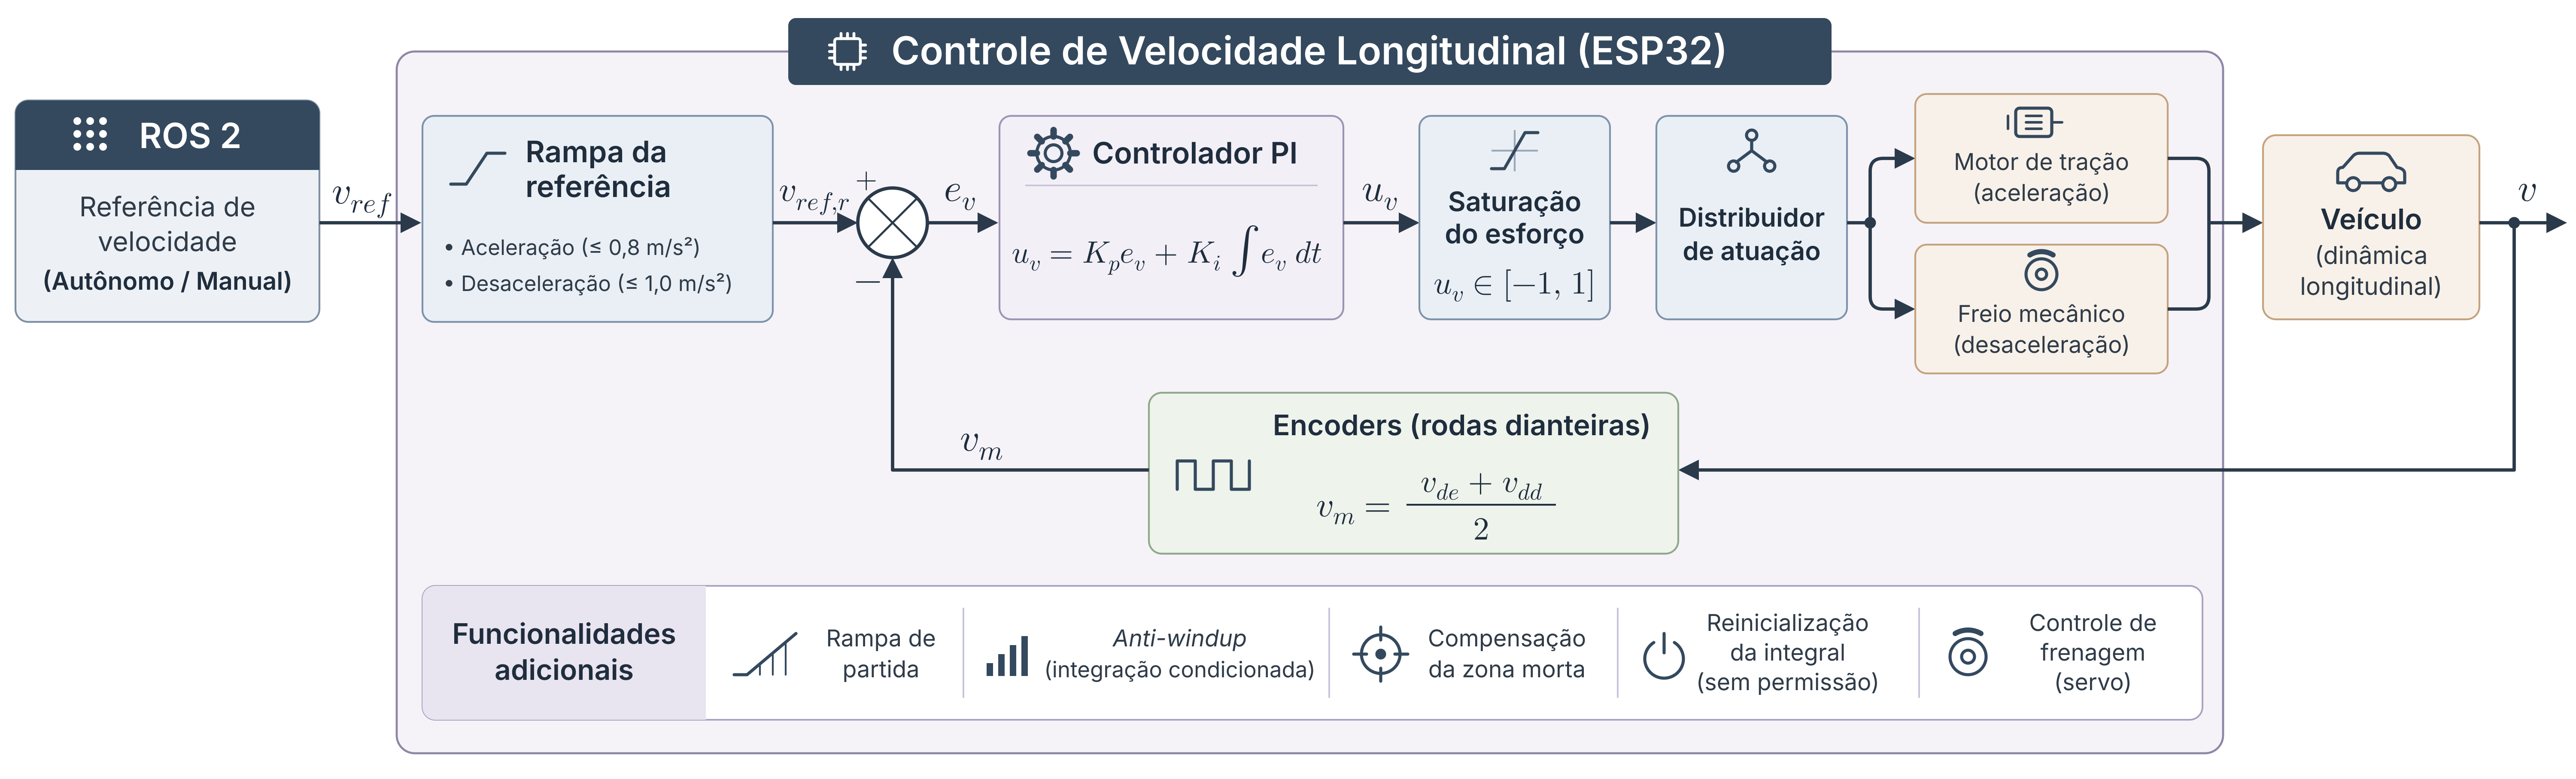
\includegraphics[width=\columnwidth]{Imagens/Malha de controle longitudinal.png}
    \caption{Diagrama da malha fechada de controle de velocidade longitudinal. Fonte: Elaborado pelo autor.}
    \label{fig:controle_velocidade}
\end{figure}

Os ganhos do controlador foram inicialmente ajustados com o auxílio de simulações e posteriormente refinados por meio de ensaios experimentais na plataforma VIDA. A Tabela~\ref{tab:parametros_controle_velocidade} apresenta os ganhos e os limites operacionais adotados na configuração utilizada durante a validação experimental.

\begin{table}[htb]
    \centering
    \caption{Parâmetros do controle de velocidade longitudinal.}
    \label{tab:parametros_controle_velocidade}
    \begin{tabular}{lc}
        \hline
        \textbf{Parâmetro} & \textbf{Valor} \\
        \hline
        Ganho proporcional ($K_p$) & 0,10 \\
        Ganho integral ($K_i$) & 0,025 \\
        Frequência de controle & 200~Hz \\
        Velocidade máxima & $2,5~\mathrm{m/s}$ \\
        Aceleração padrão & $0,4~\mathrm{m/s^2}$ \\
        Aceleração máxima & $0,8~\mathrm{m/s^2}$ \\
        Desaceleração máxima & $1,0~\mathrm{m/s^2}$ \\
        \hline
    \end{tabular}
\end{table}

\section{Estimação de Estados}
\label{sec:estimacao}

Para realizar o seguimento autônomo de trajetórias, é necessário conhecer continuamente a posição, a orientação e a velocidade do veículo. Entretanto, as medições dos sensores embarcados estão sujeitas a ruídos, incertezas e diferentes frequências de atualização. Para combinar essas informações e obter estimativas consistentes dos estados do veículo, a plataforma VIDA utiliza um filtro de Kalman estendido (EKF), executado na Odroid, cujos resultados são disponibilizados ao sistema de navegação.

\subsection{Modelo de Estados}
\label{subsec:modelo_estados}

O estimador utiliza o modelo cinemático de bicicleta, apresentado na Seção~\ref{subsec:modelo_bicicleta}, para representar a evolução do movimento do veículo. Esse modelo estabelece as relações entre posição, orientação, velocidade longitudinal e ângulo de esterçamento, permitindo prever o comportamento do sistema ao longo do tempo.

O vetor de estados considerado pelo filtro é definido por:

\begin{equation}
\mathbf{x} =
\begin{bmatrix}
x_r & y_r & \theta & \delta & v & b_g
\end{bmatrix}^{T},
\label{eq:vetor_estados_ekf}
\end{equation}

em que $x_r$ e $y_r$ representam as coordenadas da posição do veículo em um referencial global, $\theta$ corresponde à sua orientação nesse referencial, $\delta$ ao ângulo de esterçamento, $v$ à velocidade longitudinal no eixo traseiro e $b_g$ ao \textit{bias} do giroscópio.

A inclusão do \textit{bias} do giroscópio no vetor de estados permite considerar erros sistemáticos associados à medição da velocidade angular. Dessa forma, além das variáveis que descrevem o movimento do veículo, o estimador contempla uma componente destinada à compensação de desvios presentes nas medições inerciais.

A partir desse modelo, a etapa de predição do EKF propaga os estados estimados e suas respectivas incertezas ao longo do tempo. As estimativas obtidas na etapa de predição são posteriormente atualizadas por meio das medições dos sensores, conforme os princípios apresentados na Subseção~\ref{subsec:fund_ekf}.

\subsection{Fusão Sensorial e Correção dos Estados}
\label{subsec:fusao_sensorial}

A estimação dos estados é realizada por meio de ciclos sucessivos de predição e correção, combinando o modelo cinemático de bicicleta com as medições dos sensores embarcados. Na implementação utilizada no VIDA, o EKF opera a uma frequência nominal de 50~Hz, propagando continuamente a posição e a orientação do veículo. As medições de velocidade longitudinal e ângulo de esterçamento são utilizadas na predição do movimento, enquanto o giroscópio e o receptor GNSS contribuem para a atualização da orientação e a correção dos desvios de posicionamento.

Na etapa de predição, a velocidade longitudinal é obtida pela média das medições dos \textit{encoders} dianteiros, enquanto o ângulo de esterçamento é fornecido pelo LVDT. Como a velocidade considerada corresponde àquela medida nas rodas dianteiras, o modelo incorpora uma compensação geométrica para determinar o deslocamento do centro do eixo traseiro, adotado como referência de posição do veículo. Dessa forma, a propagação das coordenadas é realizada por meio das equações:

\begin{equation}
\begin{aligned}
x_{k+1}^{-} &= x_k + v_k \cos(\theta_k)\Delta t, \\
y_{k+1}^{-} &= y_k + v_k \sin(\theta_k)\Delta t.
\end{aligned}
\label{eq:predicao_posicao_ekf}
\end{equation}

Para a atualização da orientação, a implementação utiliza prioritariamente a velocidade angular medida pelo giroscópio. Durante o movimento, essa medição é corrigida pelo \textit{bias} estimado, permitindo representar a rotação do veículo sem depender exclusivamente da relação cinemática entre velocidade e esterçamento. A evolução da orientação é calculada por:

\begin{equation}
\theta_{k+1}^{-} = \theta_k + (\omega_{m,k} - b_{g,k})\Delta t,
\label{eq:predicao_orientacao_ekf}
\end{equation}

em que $\omega_{m,k}$ corresponde à velocidade angular medida pelo giroscópio e $b_{g,k}$ representa o \textit{bias} estimado. Caso as medições inerciais deixem de estar disponíveis, o estimador utiliza o modelo cinemático de bicicleta (Equação~\ref{eq:modelo_cinematico}) como alternativa para calcular a velocidade angular, o que mantém a propagação da orientação durante interrupções temporárias na
comunicação com o sensor.

O \textit{bias} do giroscópio recebe tratamento específico para reduzir o acúmulo de erros na orientação estimada. Durante a inicialização, seu valor é determinado a partir da média das medições obtidas com o veículo parado. Posteriormente, quando os \textit{encoders} indicam velocidade inferior a $0{,}02~\mathrm{m/s}$ por um período mínimo de $0{,}5~\mathrm{s}$, o estimador considera que a velocidade angular real é nula. Nessa condição, a medição do giroscópio é utilizada na etapa de correção para atualizar o \textit{bias}, enquanto a integração da orientação é interrompida, evitando a acumulação de desvios durante as paradas.

Além da propagação dos estados, o filtro incorpora as medições de velocidade e esterçamento em sua etapa de correção, atualizando as respectivas incertezas. Embora essas grandezas sejam diretamente atualizadas pelas leituras dos sensores durante a predição, sua inclusão no processo de correção permite ajustar a matriz de covariância associada ao estado estimado.

A correção do posicionamento é realizada a partir das coordenadas fornecidas pelo receptor GNSS com correções RTK. A cada nova observação válida, disponibilizada nominalmente a 2~Hz, o filtro compara a posição medida com aquela prevista pelo modelo de movimento. As diferenças identificadas são utilizadas para atualizar a estimativa por meio do ganho de Kalman, considerando as incertezas associadas às medições GNSS. Dessa forma, os desvios acumulados durante a propagação são corrigidos periodicamente, enquanto as relações representadas na matriz de covariância permitem que essas atualizações também influenciem indiretamente outros estados, como a orientação.

A combinação dessas informações permite manter estimativas regulares de posição e orientação entre as atualizações do GNSS. Durante o deslocamento, a predição utiliza as medições de velocidade, esterçamento e velocidade angular para acompanhar o movimento do veículo, enquanto as observações de posicionamento limitam o acúmulo de desvios. Nas condições de parada, a atualização do \textit{bias} do giroscópio contribui para reduzir erros sistemáticos na estimação da orientação, proporcionando maior consistência às informações disponibilizadas pelo estimador.

O estimador utilizado neste trabalho baseia-se no filtro de Kalman estendido apresentado por \citet{DeLima2015}, posteriormente adaptado à plataforma VIDA e implementado como um nó ROS~2 para realizar a fusão das medições dos sensores embarcados e estimar os estados do veículo.

\section{Seguimento de Trajetória}
\label{sec:seguimento_trajetoria}

Para validar toda a arquitetura proposta para o veículo VIDA, foi desenvolvido uma aplicação de seguimento autônomo de trajetórias realizado por meio de uma implementação do controlador Stanley, executada em um nó ROS~2 no notebook. O algoritmo utiliza os estados estimados pelo EKF e uma trajetória de referência previamente definida para calcular os comandos de esterçamento necessários à correção dos desvios de posição e orientação. A implementação incorpora modificações à formulação original, visando melhorar o comportamento do veículo durante a operação experimental.

\subsection{Implementação do Controlador Stanley}
\label{subsec:implementacao_stanley}

As trajetórias de referência são representadas por sequências de pontos geográficos, posteriormente convertidos para o referencial de navegação utilizado pelo estimador. Os pontos são tratados para produzir um caminho contínuo, com informações de orientação e curvatura necessárias ao cálculo do controle.

Para determinar os erros de seguimento, considera-se a posição do centro do eixo dianteiro, calculada a partir da posição estimada do eixo traseiro e do entre-eixos geométrico do veículo:

\begin{equation}
\begin{aligned}
x_f &= x_r + L\cos(\theta), \\
y_f &= y_r + L\sin(\theta).
\end{aligned}
\label{eq:posicao_eixo_dianteiro}
\end{equation}

em que $(x_f,y_f)$ representa a posição do centro do eixo dianteiro, $(x_r,y_r)$ corresponde à posição estimada do veículo, $\theta$ é sua orientação e $L$ representa o entre-eixos geométrico.

A posição calculada é projetada sobre a trajetória de referência, permitindo determinar o erro lateral $e$, o erro de orientação $\psi$ e a curvatura local $\kappa$ da trajetória. A partir dessas informações, o controlador calcula o ângulo de esterçamento pela seguinte expressão:

\begin{equation}
\delta =
\psi
- \arctan\left(\frac{ke}{v+k_s}\right)
+ k_{ff}\arctan(L_{ff}\kappa)
- k_r(r-v\kappa).
\label{eq:stanley_modificado}
\end{equation}

em que $k$ representa o ganho de correção lateral, $k_s$ é o parâmetro de suavização em baixas velocidades, $k_{ff}$ corresponde ao ganho antecipativo, $L_{ff}$ é o entre-eixos utilizado na compensação de curvatura, $\kappa$ representa a curvatura da trajetória de referência no ponto de projeção do eixo dianteiro, $k_r$ representa o ganho de amortecimento e $r$ corresponde à velocidade angular medida do veículo.

O primeiro termo corrige o erro de orientação, enquanto o segundo atua sobre o deslocamento lateral em relação à trajetória. Nesse termo, o parâmetro $L_{ff}$ foi ajustado experimentalmente para $1{,}17$~m, diferindo do entre-eixos geométrico do veículo ($L = 1{,}125$~m), a fim de representar melhor a relação entre esterçamento e curvatura observada na prática. O terceiro termo introduz uma ação antecipativa baseada na curvatura do caminho, permitindo considerar o esterçamento necessário à realização das curvas. Por fim, o termo de amortecimento utiliza a diferença entre a velocidade angular medida e aquela prevista pela curvatura da trajetória, contribuindo para reduzir oscilações durante o seguimento.

O comando resultante é limitado à faixa de $\pm20^\circ$ e submetido a uma restrição de taxa de variação de $40^\circ/\mathrm{s}$, evitando alterações excessivamente bruscas na referência enviada ao controlador de esterçamento. Os principais parâmetros utilizados nos ensaios experimentais são apresentados na Tabela~\ref{tab:parametros_stanley}.

\begin{table}[ht]
    \centering
    \caption{Parâmetros do controlador Stanley.}
    \label{tab:parametros_stanley}
    \begin{tabular}{lc}
        \hline
        \textbf{Parâmetro} & \textbf{Valor} \\
        \hline
        Ganho lateral ($k$) & 1,5 \\
        Suavização ($k_s$) & 1,0 m/s \\
        Ganho antecipativo ($k_{ff}$) & 1,0 \\
        Entre-eixos geométrico ($L$) & 1,125 m \\
        Entre-eixos antecipativo ($L_{ff}$) & 1,17 m \\
        Amortecimento ($k_r$) & 0,2 s \\
        Limite de esterçamento & $\pm20^\circ$ \\
        Taxa máxima de esterçamento & $40^\circ/\mathrm{s}$ \\
        Velocidade de referência & 2,0 m/s \\
        \hline
    \end{tabular}
\end{table}

O controlador utiliza uma referência de velocidade longitudinal constante durante o seguimento da trajetória. A velocidade e o ângulo de esterçamento calculados são publicados em tópicos ROS~2 específicos, posteriormente encaminhados aos controladores de baixo nível executados no ESP32.

\subsection{Gerenciamento da Navegação Autônoma}
\label{subsec:gerenciamento_navegacao}

A execução do seguimento de trajetória é supervisionada por um gerenciador de modos de operação, responsável por coordenar a condução manual e a navegação autônoma, verificando as condições necessárias ao funcionamento do sistema.

No modo manual, o operador utiliza um gamepad para controlar a velocidade longitudinal e o esterçamento do veículo por meio dos comandos analógicos, além de acionar a frenagem e solicitar a alternância entre os modos de operação. Esse controle permite posicionar o veículo próximo ao início da trajetória de referência, onde o operador solicita a ativação da navegação autônoma.

A partir dessa solicitação, o gerenciador verifica as condições de funcionamento dos subsistemas de controle e localização, incluindo a disponibilidade e a qualidade das estimativas de posicionamento, a liberação do movimento pelo ESP32 e a proximidade do veículo ao início da trajetória de referência.

Após essas verificações, o gerenciador executa uma sequência de preparação que compreende o alinhamento das rodas dianteiras, a reinicialização do estimador de estados e um deslocamento inicial em linha reta para o estabelecimento da orientação de navegação. Durante esse deslocamento, assim que a orientação é estabelecida e as condições de alinhamento com a trajetória de referência são atendidas, o controlador Stanley assume o comando de esterçamento, dando continuidade ao movimento em modo autônomo.

Durante a operação autônoma, o gerenciador monitora continuamente a disponibilidade das informações de localização, a comunicação com os sistemas embarcados e os desvios em relação à trajetória. Condições consideradas inadequadas, como perda de informações essenciais, erros laterais excessivos ou intervenção do operador, provocam a interrupção do seguimento autônomo.

Ao se aproximar do ponto final da trajetória, o gerenciador inicia o procedimento de frenagem, reduzindo progressivamente a velocidade até a parada completa do veículo.
\section{Interface de Operação}
\label{subsec:painel_operacao}

\begin{figure*}[t]
    \centering
    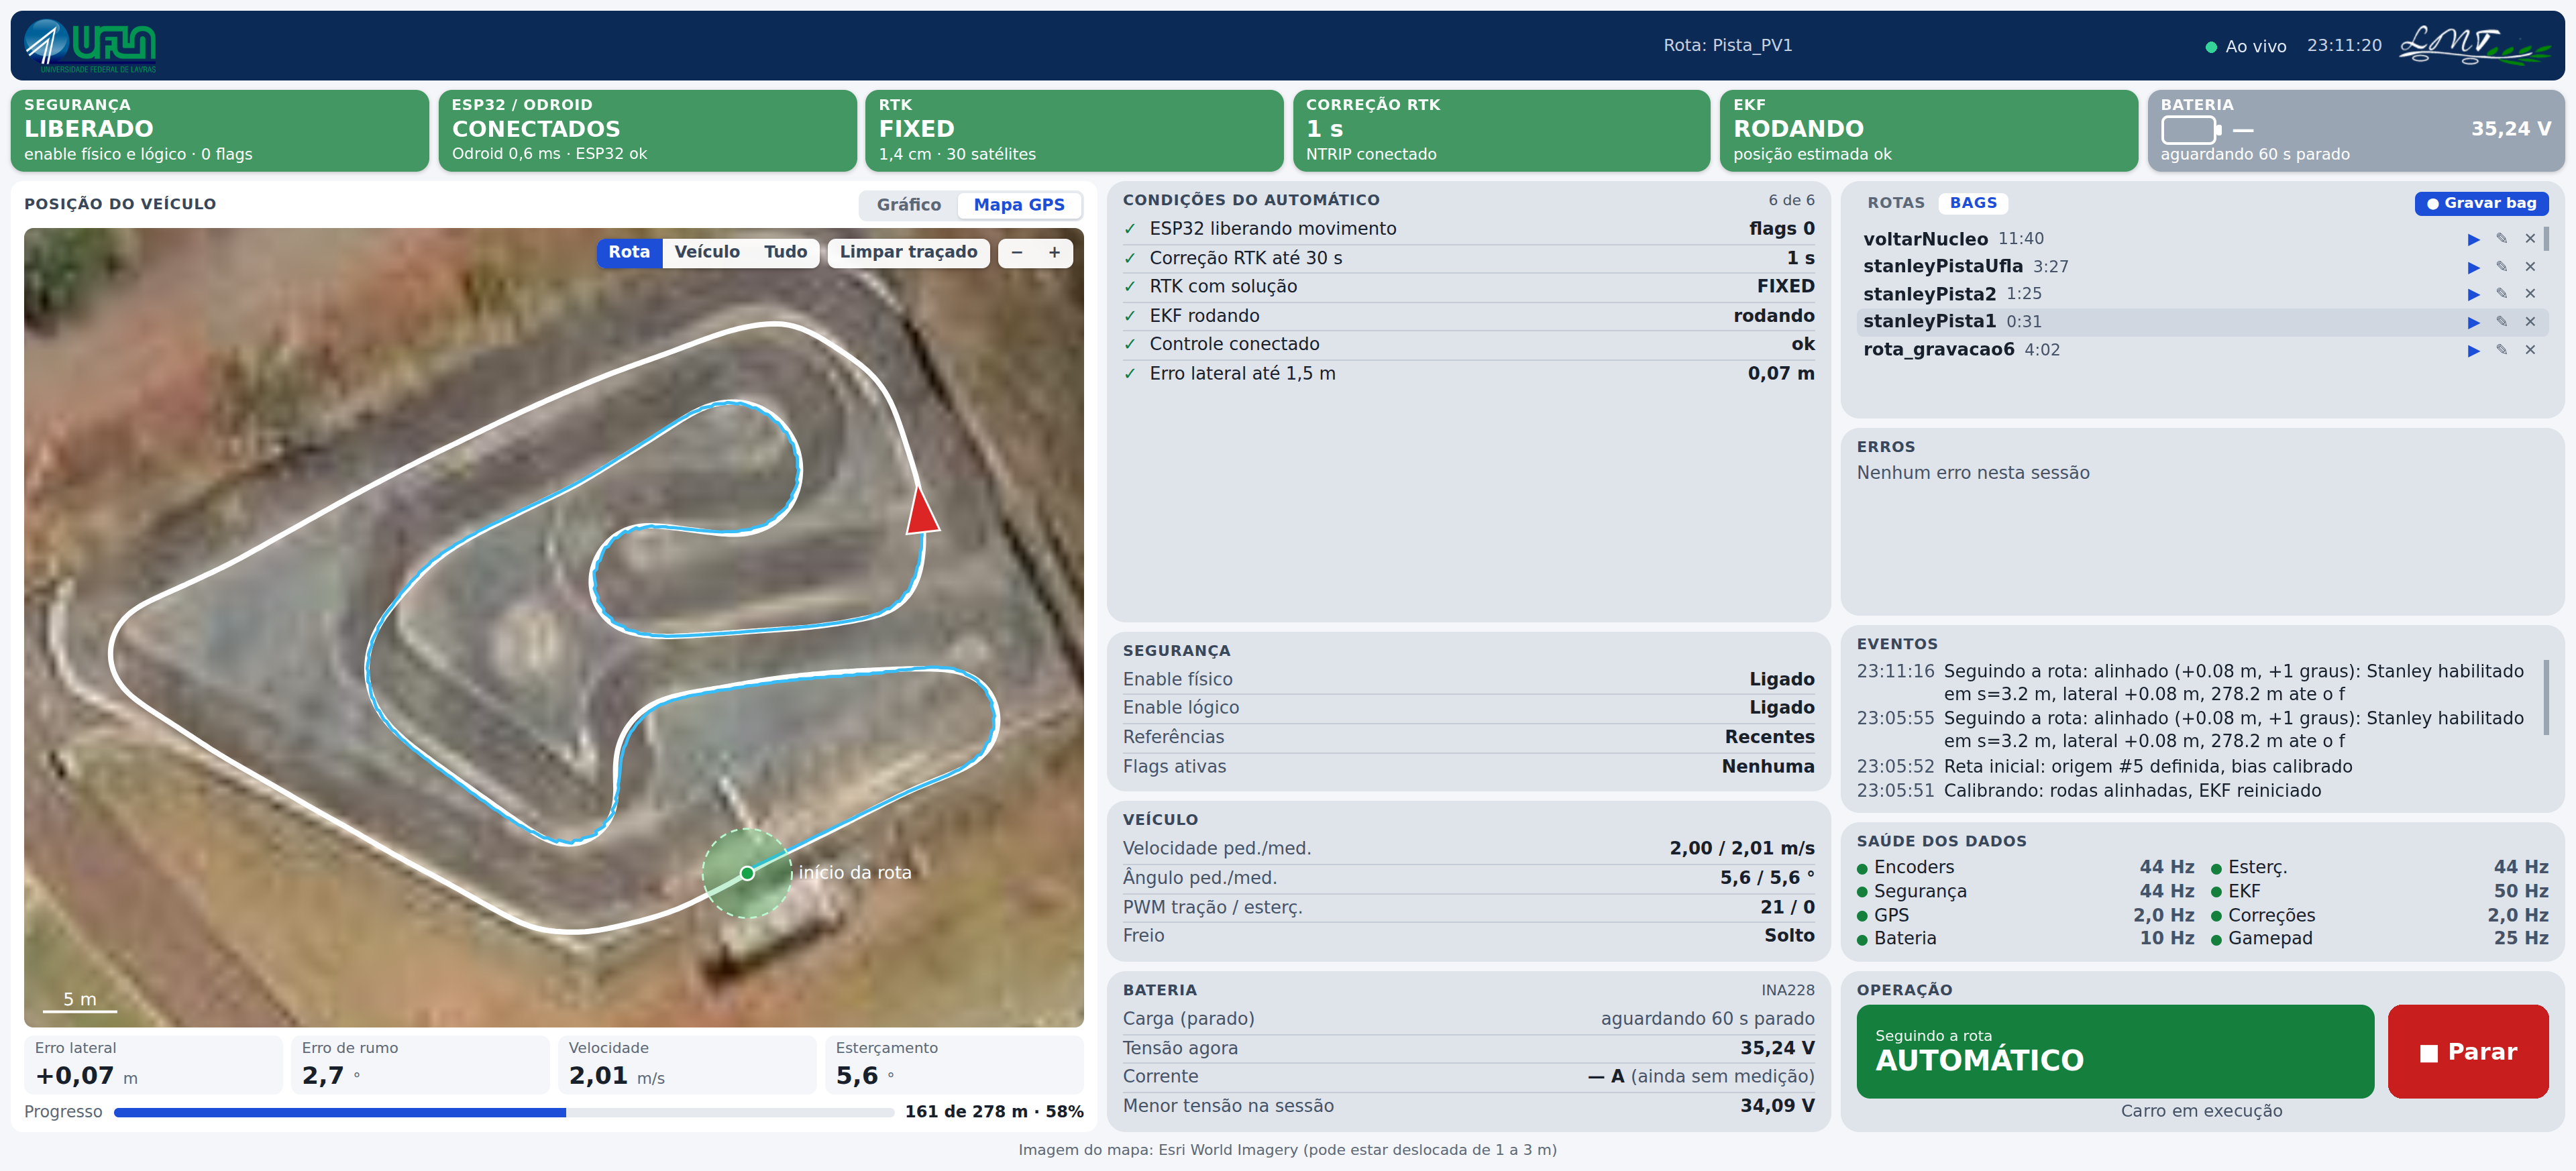
\includegraphics[width=0.98\textwidth]{Imagens/Painel_de_operacao.png}
    % legenda centralizada apenas nesta figura
    \makeatletter
    \long\def\@makecaption#1#2{\vskip 8\p@\par{\centering\@fignumfont{#1}. #2\par}}
    \makeatother
    \caption{Interface de operação e monitoramento da plataforma VIDA. Fonte: Elaborado pelo autor.}
    \label{fig:painel_operacao}
    \vspace{8pt}
\end{figure*}

Para facilitar a operação e o acompanhamento dos subsistemas da plataforma VIDA, foi desenvolvida uma interface web de supervisão, executada em um contêiner Docker no notebook de operação. O painel utiliza um servidor HTTP e  realiza atualizações periódicas via WebSocket com um nó ROS~2, que assina os tópicos de interesse e encaminha as informações à página exibida no navegador. Dessa forma, a supervisão do veículo dispensa ferramentas de visualização específicas do ROS~2 e pode ser realizada pelo próprio operador durante os ensaios.

A interface reúne, em uma única tela, informações essenciais à operação do veículo, incluindo o estado dos sistemas de segurança, condições de posicionamento GNSS/RTK, e estado do estimador de Kalman. Também permite visualizar a posição e a orientação do veículo sobre a trajetória de referência, acompanhar o progresso da navegação e consultar registros de eventos, erros e indicadores de comunicação dos subsistemas.

Além do monitoramento, o painel disponibiliza funcionalidades para iniciar e encerrar os programas de navegação, selecionar e registrar trajetórias e realizar a gravação e reprodução de dados experimentais.

A Figura~\ref{fig:painel_operacao} apresenta a interface desenvolvida, destacando a visualização da trajetória e os principais indicadores de operação e monitoramento. A centralização dessas funções em uma única interface reduz a necessidade de comandos em terminal durante os experimentos e facilita a identificação de falhas, contribuindo para a segurança e a agilidade dos ensaios.

\section{Resultados Experimentais}
\label{sec:resultados_experimentais}

A validação experimental do sistema de navegação autônoma desenvolvido para a plataforma VIDA foi realizada por meio de ensaios em ambiente real, buscando avaliar a integração dos subsistemas de sensoriamento, estimação de estados, controle de baixo nível e seguimento de trajetórias. Os experimentos permitiram verificar o funcionamento da arquitetura computacional distribuída e avaliar o comportamento do veículo durante a execução autônoma de percursos previamente definidos.

Foram realizados dois experimentos de seguimento autônomo de trajetória, denominados Trajeto 1 e Trajeto 2. A avaliação foi conduzida a partir dos dados registrados pelo ROS~2, considerando as trajetórias de referência e executadas, os erros de seguimento, os comandos de controle e as informações disponibilizadas pelo estimador de estados.

\subsection{Procedimento Experimental}
\label{subsec:procedimento_experimental}

Os ensaios foram realizados com a plataforma VIDA, utilizando os subsistemas de controle, localização e navegação apresentados nas seções anteriores.

As trajetórias de referência foram obtidas a partir de coordenadas geográficas registradas pelo receptor GNSS durante a condução manual do veículo. Os pontos coletados foram posteriormente processados por meio de suavização e reamostragem, resultando em trajetórias com espaçamento uniforme de 0,25~m, armazenadas em arquivos CSV e utilizadas pelo sistema de navegação autônoma.

A preparação e o acompanhamento dos experimentos foram realizados com o auxílio do painel de operação e monitoramento apresentado na Seção~\ref{subsec:painel_operacao}. Por meio dessa interface, foi possível selecionar as trajetórias de referência, gerenciar a inicialização dos programas de navegação e acompanhar, em tempo real, as condições de segurança, localização e controle do veículo ao longo da execução dos percursos.

O desempenho dos controladores de baixo nível foi avaliado por meio da comparação entre as referências de velocidade longitudinal e ângulo de esterçamento e as respectivas respostas medidas durante os ensaios.

Em ambos os experimentos, foi utilizada uma referência de velocidade longitudinal de 2,0~m/s. Para a avaliação quantitativa do desempenho do seguimento, foram considerados o erro médio absoluto (MAE), a raiz do erro quadrático médio (RMSE) e o erro máximo absoluto, calculados a partir dos erros laterais registrados no decorrer da navegação autônoma:

\begin{equation}
    \mathrm{MAE} = \frac{1}{N}\sum_{i=1}^{N}|e_i|,
    \label{eq:mae}
\end{equation}

\begin{equation}
    \mathrm{RMSE} = \sqrt{\frac{1}{N}\sum_{i=1}^{N}e_i^2},
    \label{eq:rmse}
\end{equation}

\begin{equation}
    e_{\mathrm{max}} = \max_{1 \leq i \leq N}|e_i|,
    \label{eq:erro_maximo}
\end{equation}

em que $e_i$ representa o erro lateral registrado em cada amostra e $N$ corresponde ao número total de amostras consideradas. O erro máximo absoluto corresponde ao maior valor de $|e_i|$ observado durante cada experimento.


\subsection{Desempenho dos Controladores de Baixo Nível}
\label{subsec:resultados_baixo_nivel}

Os controladores de baixo nível desempenham um papel fundamental na execução dos comandos de navegação, sendo responsáveis por regular o ângulo de esterçamento e a velocidade longitudinal do veículo. Sua avaliação experimental busca verificar a capacidade de acompanhar as referências estabelecidas, bem como identificar possíveis limitações associadas à dinâmica dos atuadores. Os resultados são apresentados a seguir, iniciando pela malha de esterçamento e, posteriormente, pela malha de velocidade longitudinal.

O controlador PID de esterçamento apresentou capacidade de acompanhar as referências angulares fornecidas pelo controlador Stanley durante o seguimento autônomo de trajetória. Conforme apresentado na Figura~\ref{fig:resposta_esterçamento}, o ângulo medido pelo sensor LVDT acompanhou as variações da referência, apresentando RMSE de 1,68$^\circ$ e atraso estimado de aproximadamente 175~ms. Esse atraso pode estar associado à combinação de fatores como a filtragem do sinal do LVDT, a latência da comunicação entre os dispositivos, o atrito do mecanismo de direção e a zona morta do controlador. O erro máximo absoluto registrado foi de 4,47$^\circ$, observado após uma curva mais fechada à direita, quando a referência de esterçamento variou rapidamente de aproximadamente 20$^\circ$ para $-20^\circ$.

\begin{figure}[htb]
    \centering
    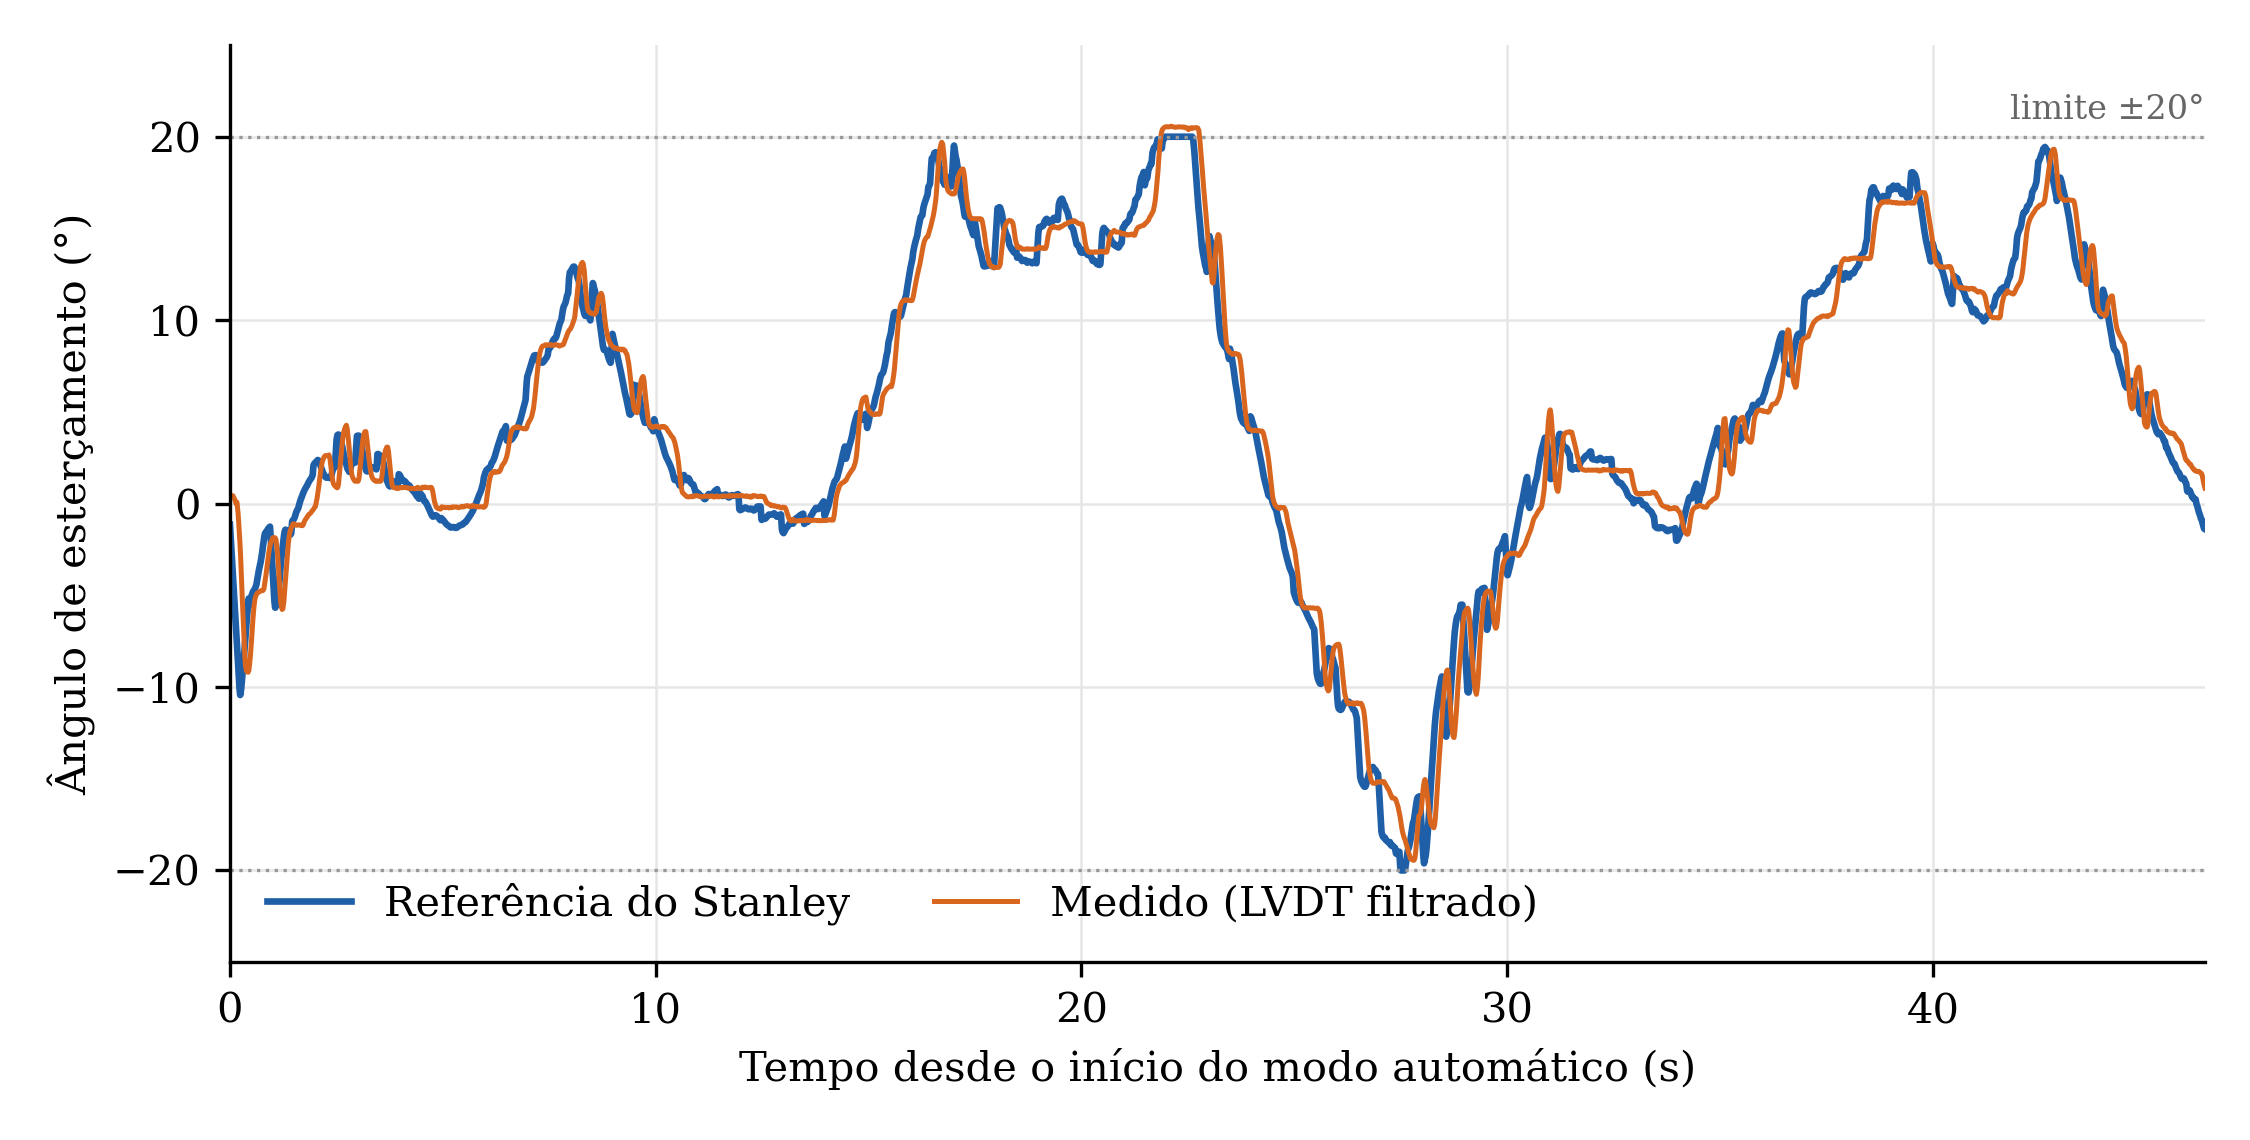
\includegraphics[width=\columnwidth]{Imagens/Resposta PID esterçamento.png}
    \caption{Resposta experimental do controlador de esterçamento. Fonte: Elaborado pelo autor.}
    \label{fig:resposta_esterçamento}
\end{figure}

Observa-se também que a resposta apresenta pequenos movimentos em degraus, especialmente durante variações reduzidas da referência. Esse comportamento resulta da interação entre a zona morta implementada no controlador, o atrito estático do mecanismo de direção e a ação integral. Enquanto o erro permanece dentro da zona morta, o acionamento é interrompido e o estado integral é mantido nulo.

Quando o erro excede esse limite e o atrito estático impede o movimento, a parcela integral aumenta progressivamente até que o esforço de controle seja suficiente para iniciar o deslocamento, que ocorre rapidamente até as proximidades da referência. Esse ciclo de adesão e deslizamento (\textit{stick-slip}) é característico de sistemas com atrito estático submetidos a controladores com ação integral. Como o estado integral é reinicializado na zona morta e ao cruzar a referência, além de ser limitado em amplitude, o esforço acumulado não se propaga entre ciclos consecutivos.

Por sua vez, o controlador PI de velocidade longitudinal foi avaliado quanto à capacidade de manter a velocidade do veículo próxima à referência de 2,0~m/s ao longo do seguimento autônomo de trajetória. Conforme apresentado na Figura~\ref{fig:resposta_velocidade}, a velocidade medida apresentou pequenas oscilações em torno da referência. Em regime permanente, a velocidade média foi de 1,998~m/s, com RMSE de 0,063~m/s, equivalente a aproximadamente 3,2\% da velocidade de referência. O erro máximo absoluto registrado foi de 0,187~m/s.

\begin{figure}[htb]
    \centering
    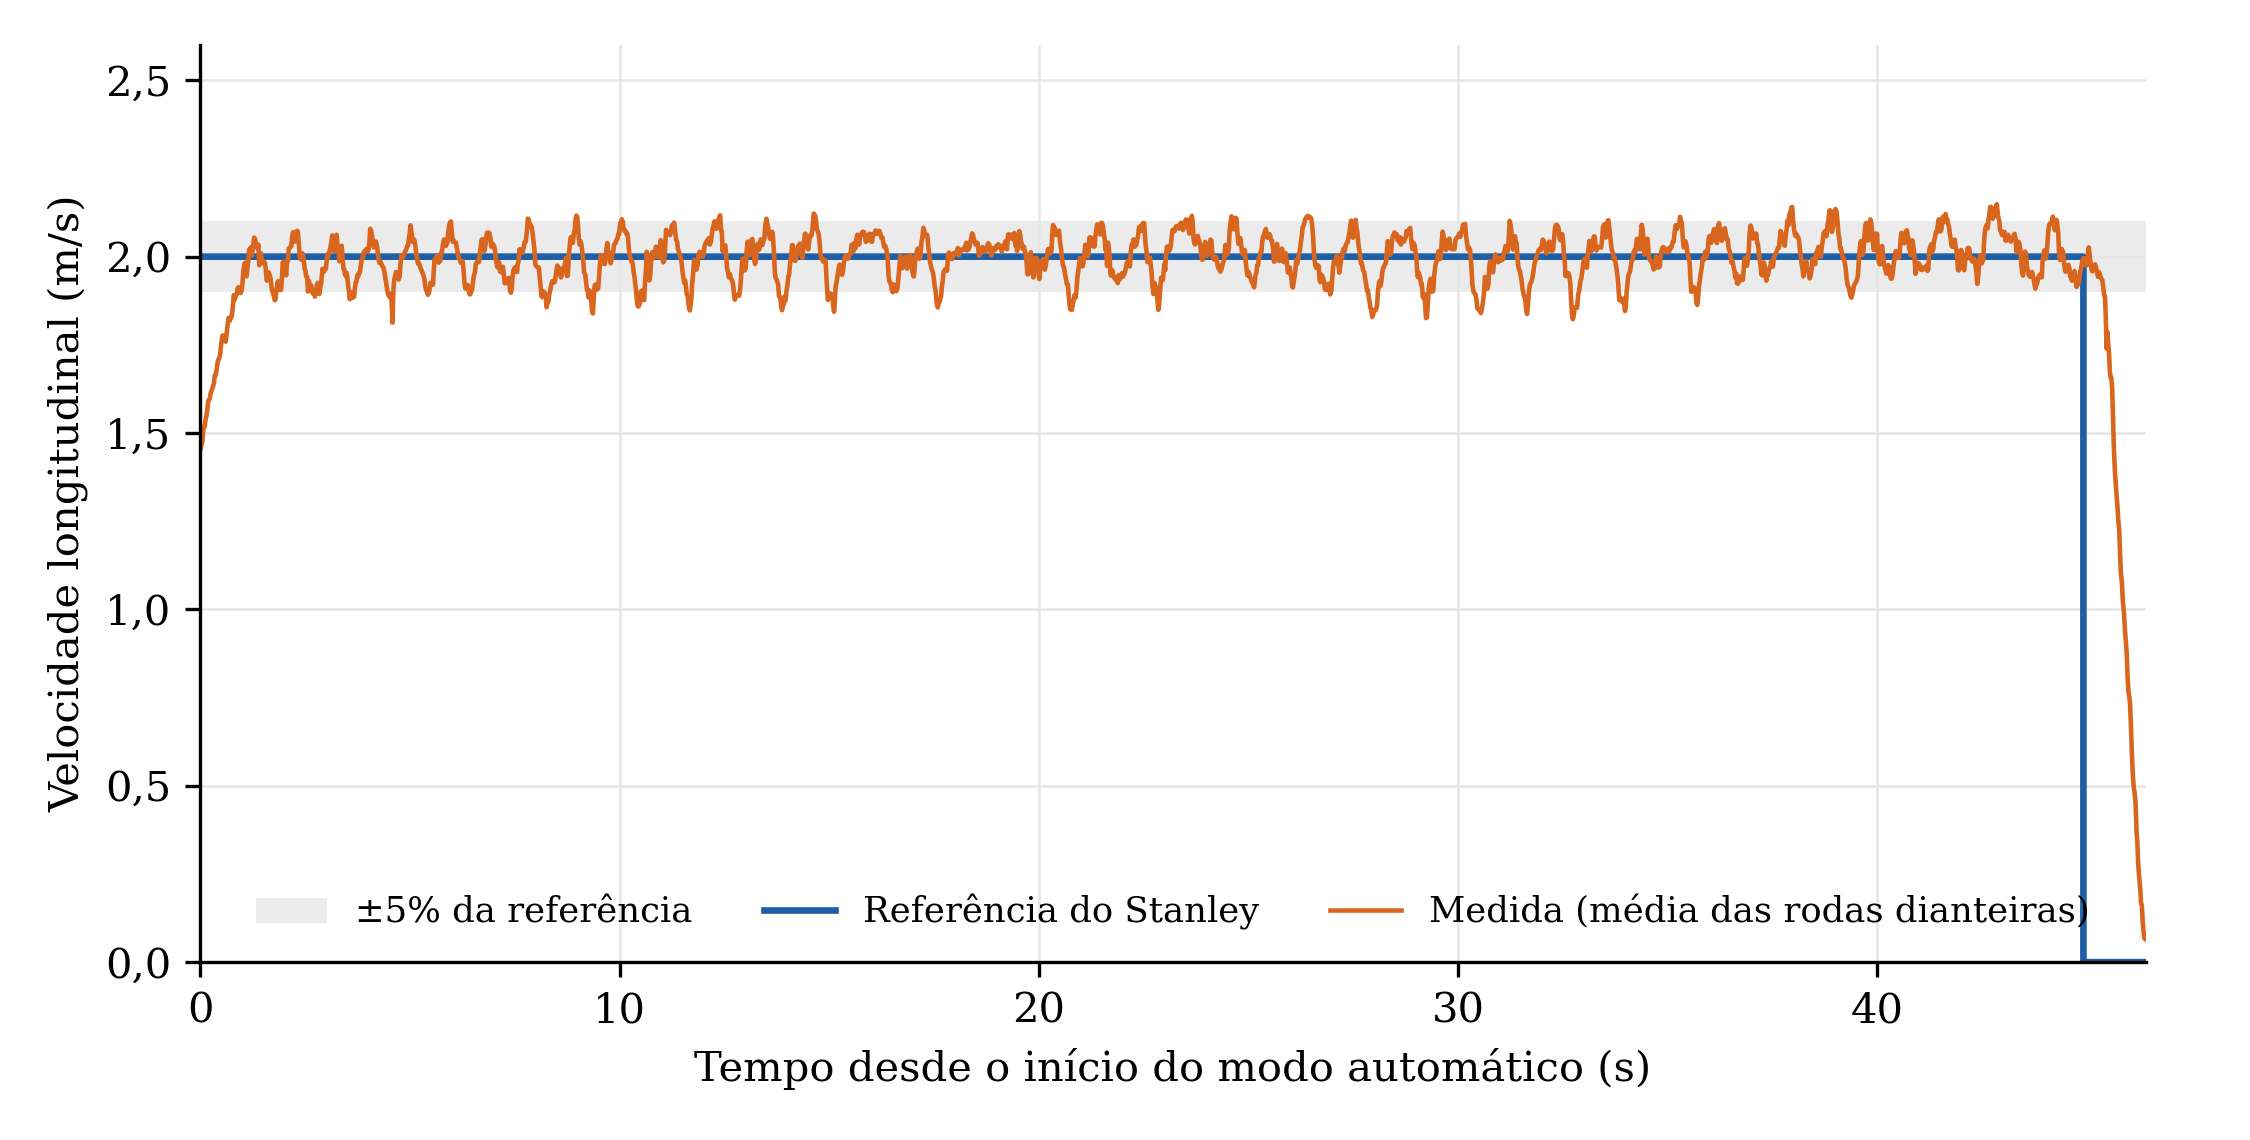
\includegraphics[width=\columnwidth]{Imagens/Resposta PI velocidadade longitudinal.png}
    \caption{Resposta experimental do controlador de velocidade longitudinal. Fonte: Elaborado pelo autor.}
    \label{fig:resposta_velocidade}
\end{figure}

As oscilações observadas estão relacionadas à zona morta de acionamento do motor, que exige um sinal PWM mínimo de aproximadamente 7,8\% para produzir o acionamento do módulo de conversão de potência. Entretanto, o acionamento médio necessário para manter a velocidade de referência corresponde a aproximadamente 7,5\% do PWM. Dessa forma, o menor acionamento disponível produz uma aceleração superior à necessária, fazendo com que a velocidade ultrapasse a referência. O controlador PI então interrompe a tração, permitindo que o veículo desacelere naturalmente devido às resistências ao movimento. Quando a velocidade retorna a valores inferiores à referência, a tração é restabelecida, produzindo oscilações periódicas em torno da velocidade desejada. A análise da saída do controlador confirma esse comportamento: em regime, o PWM de tração permaneceu entre 20 e 26, distante do limite de saturação de 50, e o freio não foi acionado. A parcela integral manteve-se aproximadamente constante, enquanto a oscilação do esforço de controle foi conduzida pela parcela proporcional, indicando que o fenômeno decorre da zona morta do acionamento, e não do acúmulo da ação integral. A Figura~\ref{fig:pwm_parcelas_pi_velocidade} apresenta o comportamento do PWM aplicado e das parcelas proporcional e integral do controlador em regime permanente.

\begin{figure}[htb]
    \centering
    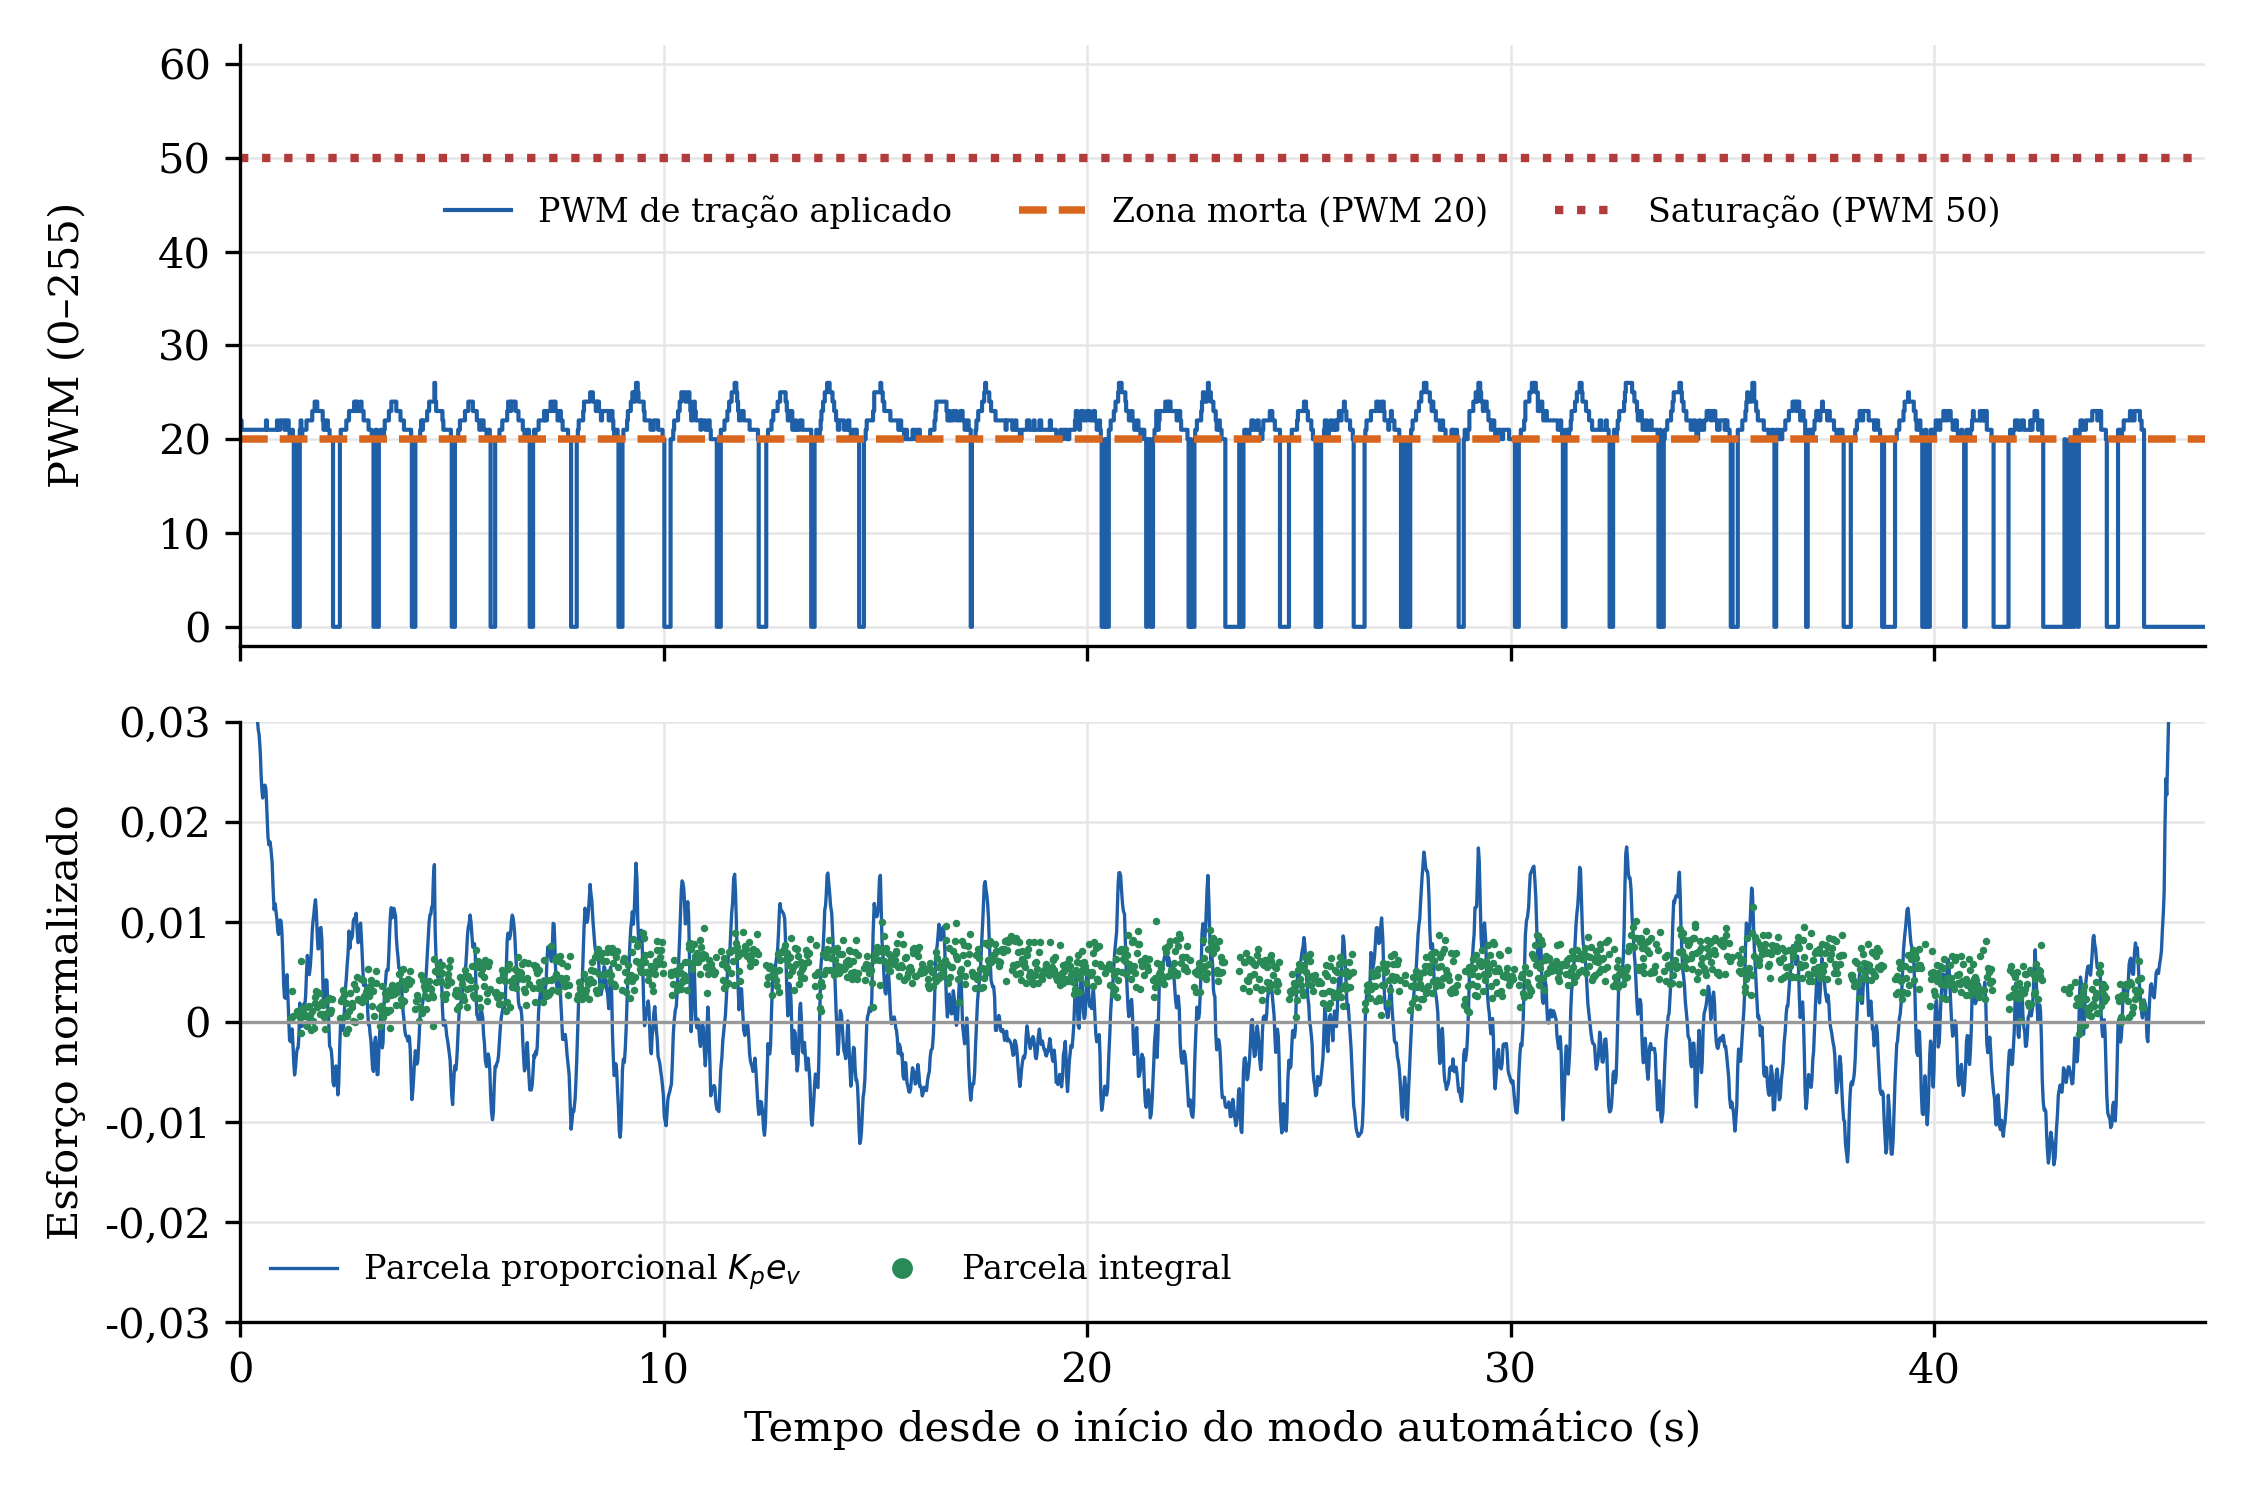
\includegraphics[width=\columnwidth]{Imagens/pwm_parcelas_pi_velocidade.png}
    \caption{Análise da saída do controlador PI de velocidade longitudinal e parcelas de controle. Fonte: Elaborado pelo autor.}
    \label{fig:pwm_parcelas_pi_velocidade}
\end{figure}

Apesar dessas oscilações, o controlador apresentou desempenho satisfatório na manutenção da velocidade longitudinal. Em regime permanente, o veículo permaneceu 88,6\% do tempo dentro de uma faixa de tolerância de $\pm 5\%$ em relação à referência e 100\% do tempo dentro de $\pm 10\%$. Esse comportamento é favorecido pela inércia do veículo, que suaviza as variações de velocidade provocadas pelos acionamentos intermitentes do motor de tração.


\subsection{Seguimento de Trajetória: Trajeto 1}

O primeiro ensaio de seguimento autônomo de trajetória foi realizado em um estacionamento localizado nas proximidades do Departamento de Engenharia de Alimentos da Universidade Federal de Lavras (UFLA). O local apresenta uma área aberta, favorável à recepção dos sinais GNSS e à realização dos experimentos com a plataforma VIDA.

No ensaio, o veículo percorreu aproximadamente 89~m em modo automático, ao longo de 46,5~s, mantendo velocidade média de 1,97~m/s, próxima à referência de 2,0~m/s. A Figura~\ref{fig:trajeto_1} apresenta a comparação entre a trajetória de referência e o percurso realizado pelo veículo.


\begin{figure}[htb]
    \centering
    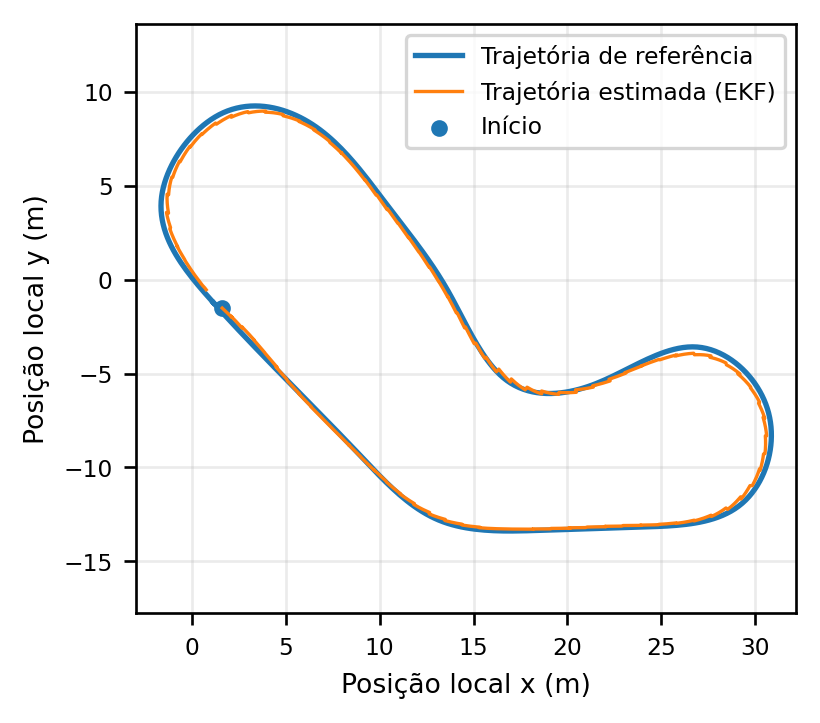
\includegraphics[width=\columnwidth]{Imagens/Trajetoria_Troia.png}
    \caption{Comparação entre a trajetória de referência e a trajetória percorrida pelo veículo no Trajeto 1. Fonte: Elaborado pelo autor.}
    \label{fig:trajeto_1}
\end{figure}

A avaliação do desempenho do controlador Stanley foi realizada a partir do erro lateral de seguimento. A Figura~\ref{fig:erro_lateral_trajeto_1} apresenta a evolução desse erro durante o percurso.

\begin{figure}[htb]
    \centering
    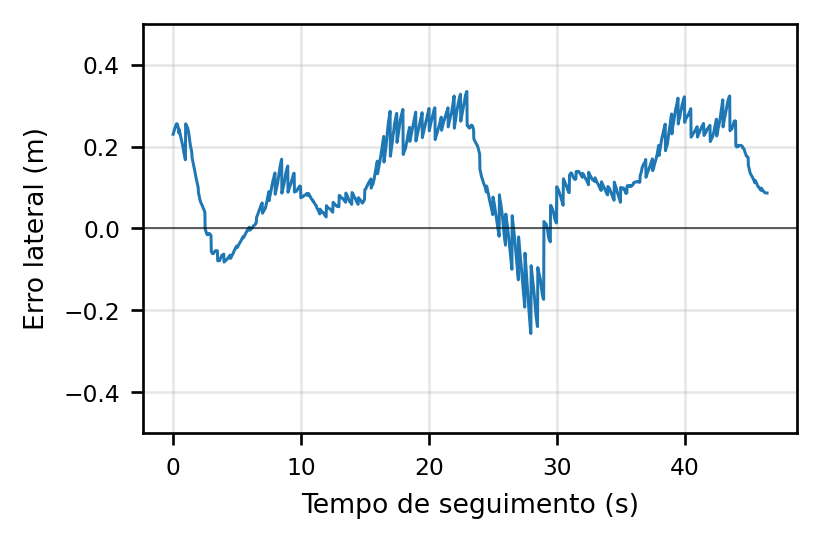
\includegraphics[width=0.85\columnwidth]{Imagens/Erro_Lateral_Troia.png}
    \caption{Evolução do erro lateral de seguimento durante o Trajeto 1. Fonte: Elaborado pelo autor.}
    \label{fig:erro_lateral_trajeto_1}
\end{figure}

O erro lateral apresentou raiz do erro quadrático médio (RMSE) de 0,167~m e valor máximo absoluto de 0,33~m. Observa-se também que o erro lateral apresenta, em alguns trechos, um padrão em dentes de serra, em vez de uma variação suave. Esse comportamento está associado ao processo de fusão de sensores do estimador de estados. Entre duas medições consecutivas do receptor GNSS, recebidas a 2~Hz, a posição do veículo é propagada pelo modelo de predição a partir da odometria, do ângulo de esterçamento e do giroscópio, acumulando um pequeno desvio que faz o erro lateral variar gradualmente. A cada nova medição GNSS, a etapa de correção reposiciona a estimativa, produzindo uma variação abrupta do erro. A análise dos registros confirma essa relação: o erro lateral apresenta uma componente periódica de 2~Hz, coincidente com a frequência de atualização do receptor GNSS, e as variações abruptas ocorrem, em média, cerca de 12~ms após a chegada de cada medição. Como essas variações ocorrem sempre no mesmo sentido, elas indicam um pequeno desvio sistemático do modelo de predição em relação às medições GNSS, possivelmente associado a erros de escala na velocidade medida ou de calibração do ângulo de esterçamento. 

Os resultados indicam que o controlador Stanley foi capaz de conduzir a plataforma VIDA ao longo da trajetória estabelecida, mantendo desvios laterais relativamente pequenos durante o percurso. Dessa forma, o ensaio demonstrou o funcionamento integrado dos subsistemas de localização, navegação e controle no seguimento automático de trajetória. A partir desse resultado, foi realizado um segundo ensaio em um percurso mais extenso, apresentado a seguir.



\subsection{Seguimento de Trajetória: Trajeto 2}
\label{subsec:trajeto_2}

O segundo ensaio de seguimento autônomo de trajetória foi realizado no autódromo da Universidade Federal de Lavras (UFLA), utilizando um percurso mais extenso e com diferentes características geométricas em relação ao primeiro experimento. A trajetória apresenta curvas e mudanças de direção, permitindo avaliar o desempenho do controlador Stanley em meio à execução de manobras sucessivas. Assim como no Trajeto 1, foram mantidos os parâmetros do controlador apresentados na Tabela~\ref{tab:parametros_stanley}, de modo que os dois ensaios fossem realizados sob a mesma configuração.

\begin{figure}[htb]
    \centering
    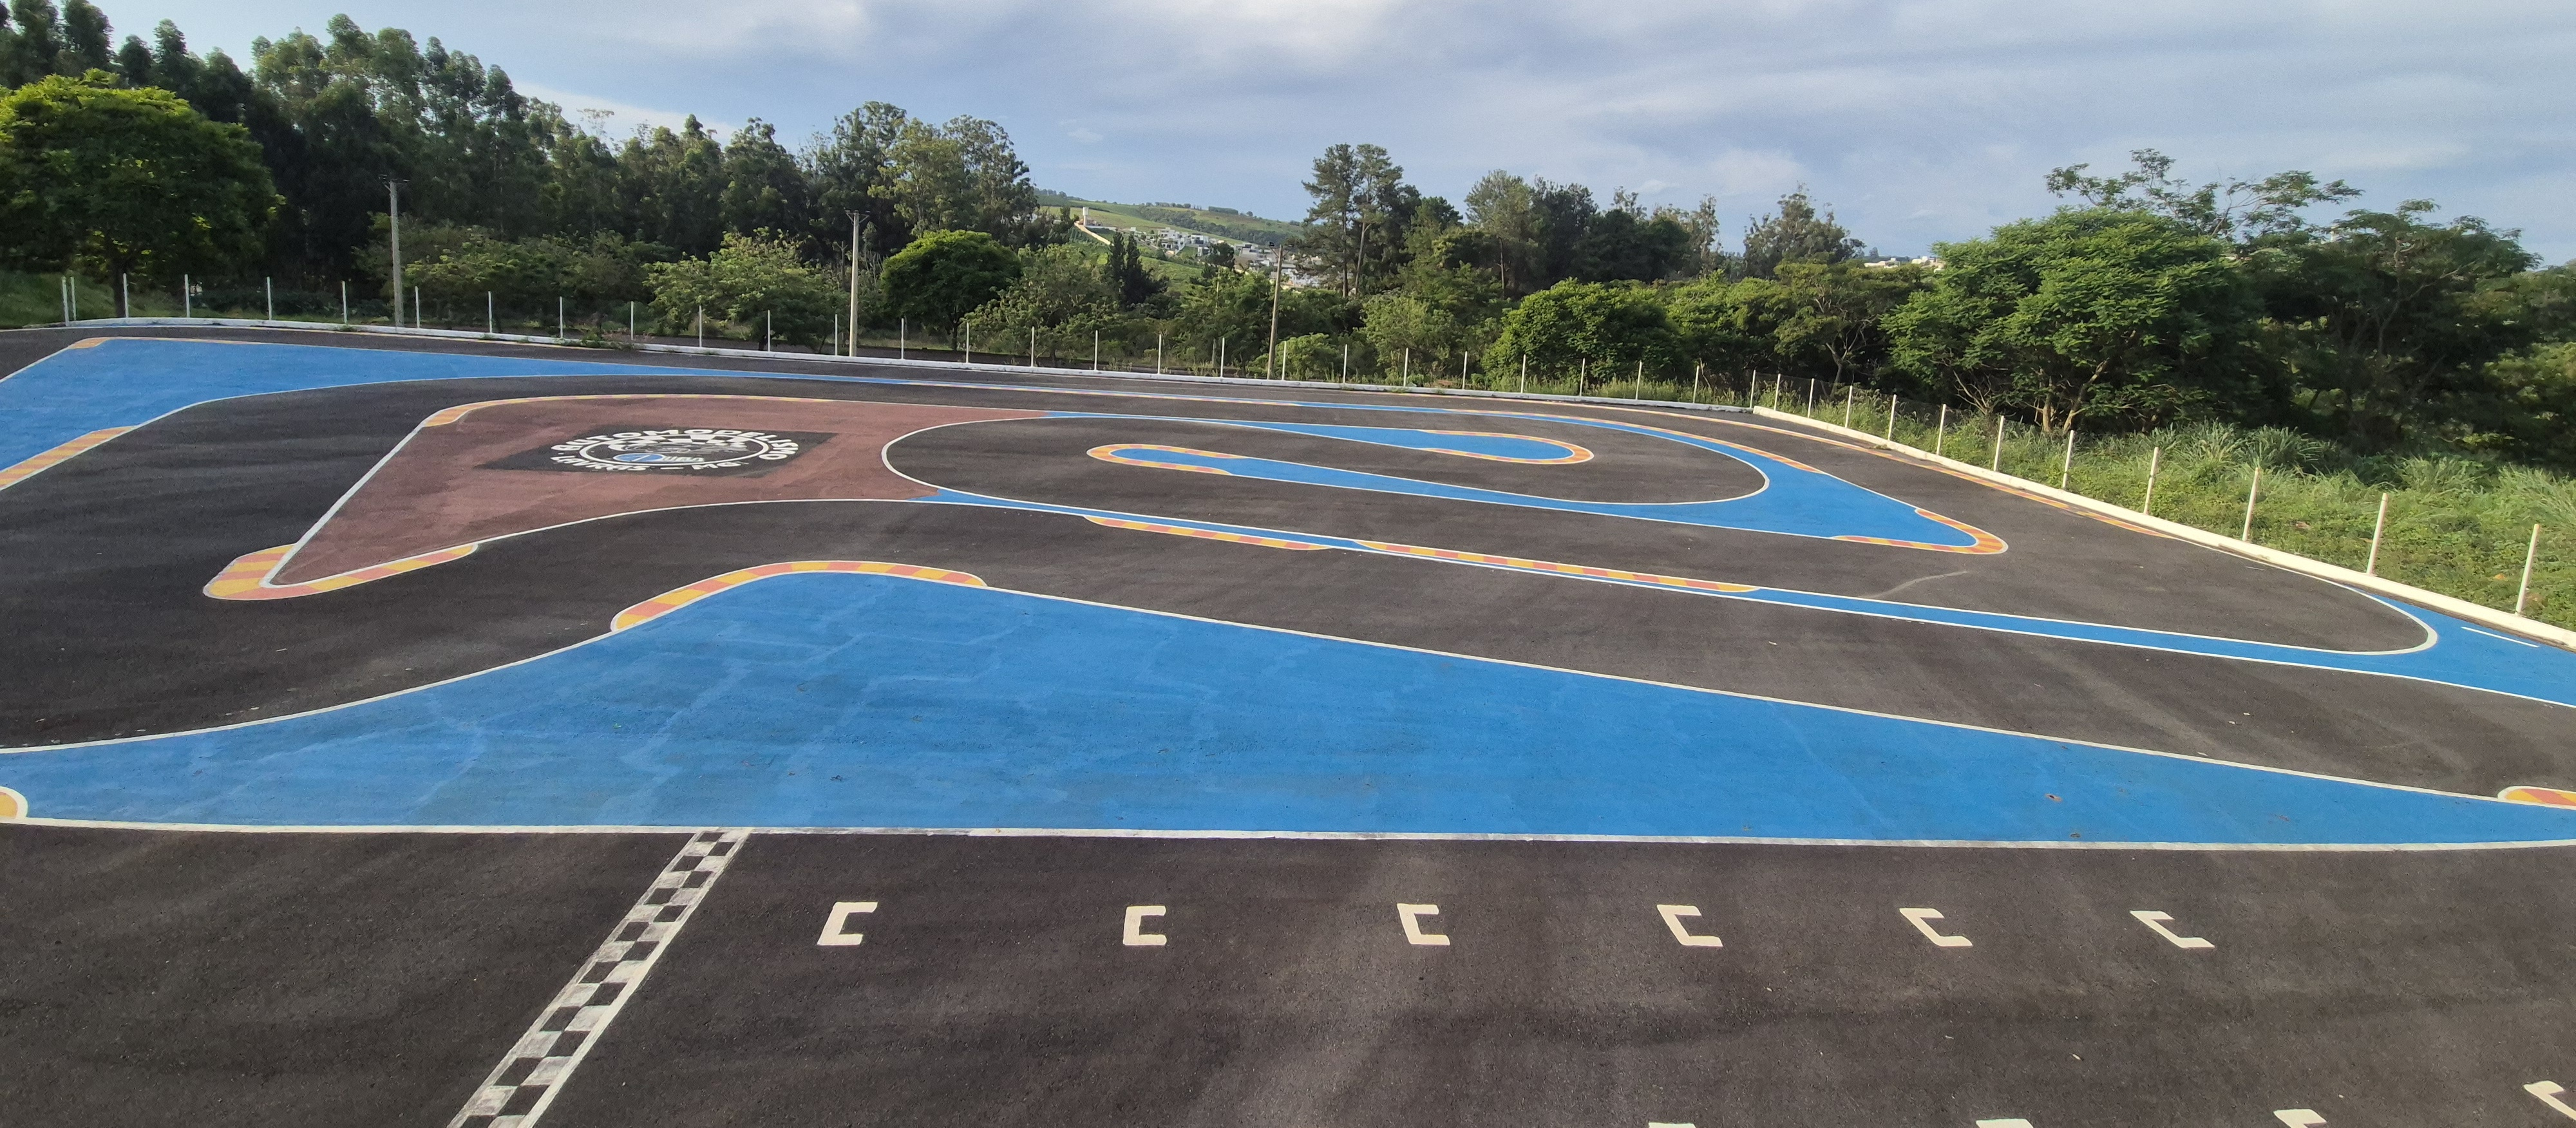
\includegraphics[width=\columnwidth]{Imagens/Autodromo_UFLA.jpg}
    \caption{Vista geral do autódromo da Universidade Federal de Lavras, utilizado no ensaio de seguimento autônomo de trajetória do Trajeto 2. Fonte: Acervo do autor.}
    \label{fig:pista_trajeto_2}
    
\end{figure}

O veículo percorreu de forma autônoma aproximadamente 281,42~m ao longo de 146,56~s, utilizando uma velocidade de referência de 2,0~m/s. A Figura~\ref{fig:trajeto_2} apresenta a comparação entre a trajetória de referência e o percurso realizado pelo veículo.

\begin{figure}[htb]
    \centering
    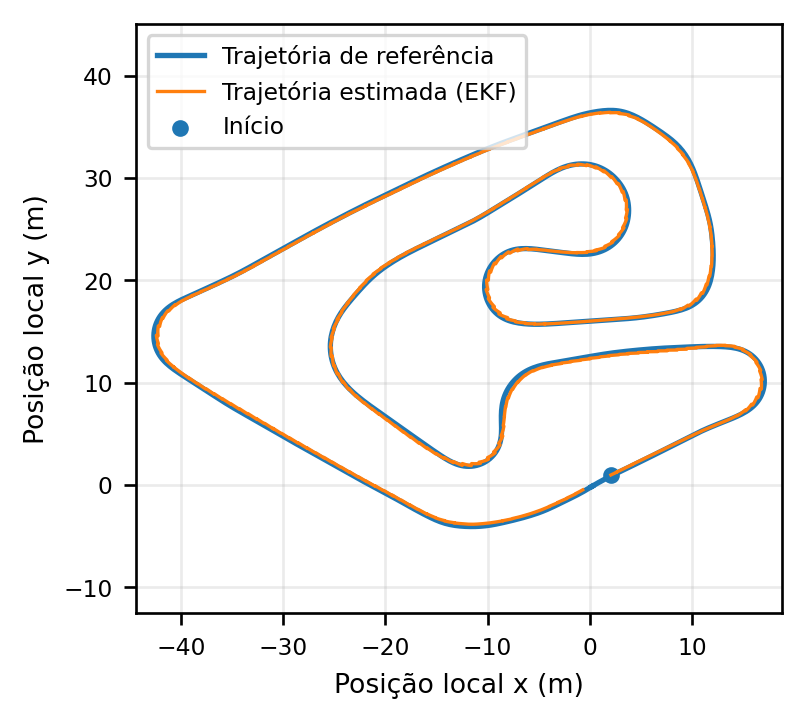
\includegraphics[width=\columnwidth]{Imagens/Trajetoria_Pista3.png}
    \caption{Comparação entre a trajetória de referência e a trajetória percorrida pelo veículo no Trajeto 2. Fonte: Elaborado pelo autor.}
    \label{fig:trajeto_2}
    
\end{figure}

Observa-se que o veículo foi capaz de acompanhar a trajetória estabelecida ao longo do percurso, realizando as correções de esterçamento necessárias para compensar os desvios laterais e de orientação. A execução desse experimento é particularmente relevante por envolver um trajeto mais extenso, exigindo a atuação contínua do controlador em diferentes condições de curvatura. A Figura~\ref{fig:erro_lateral_trajeto_2} apresenta a evolução temporal do erro lateral de seguimento durante o Trajeto 2.

\begin{figure}[htb]
    \centering
    \includegraphics[width=0.85\columnwidth]{Imagens/erro_lateral_Pista3.png}
    \caption{Evolução do erro lateral de seguimento durante o Trajeto 2. Fonte: Elaborado pelo autor.}
    \label{fig:erro_lateral_trajeto_2}
\end{figure}

Ao longo do experimento, o erro lateral médio absoluto (MAE) foi de 0,108~m, enquanto a raiz do erro quadrático médio (RMSE) apresentou valor de 0,129~m. O maior erro absoluto registrado foi de aproximadamente 0,366~m.

Esses resultados demonstram que o controlador Stanley foi capaz de manter o veículo próximo à trajetória de referência, mesmo diante das diferentes condições geométricas do percurso. Ao final do trajeto, o sistema de navegação identificou a conclusão da trajetória e realizou a transição para a condição de parada, evidenciando o funcionamento integrado dos sistemas de localização, navegação e controle da plataforma VIDA.

\subsection{Análise Comparativa dos Experimentos}

Os resultados quantitativos obtidos nos dois experimentos são apresentados na Tabela~\ref{tab:resultados_seguimento}. As métricas correspondem aos períodos de navegação autônoma identificados nos registros experimentais.

\begin{table}[htb]
    \centering
    \caption{Resultados experimentais do seguimento autônomo de trajetórias.}
    \label{tab:resultados_seguimento}
    \begin{tabular}{lcc}
        \hline
        \textbf{Métrica} & \textbf{Trajeto 1} & \textbf{Trajeto 2} \\
        \hline
        Percurso (m) & 89,24 & 281,42 \\
        Duração (s) & 46,48 & 146,56 \\
        MAE lateral (m) & 0,143 & 0,108 \\
        RMSE lateral (m) & 0,167 & 0,129 \\
        Erro máximo (m) & 0,334 & 0,366 \\
        Velocidade ref. (m/s) & 2,0 & 2,0 \\
        \hline
    \end{tabular}
\end{table}

A comparação demonstra que o sistema foi capaz de executar autonomamente dois percursos com diferentes comprimentos e características geométricas. O segundo experimento apresentou uma trajetória de referência com comprimento correspondente a aproximadamente 3,15 vezes o comprimento da primeira, mantendo valores reduzidos de erro lateral ao longo da execução.

No Trajeto 1, o RMSE lateral foi de 0,167~m, enquanto no Trajeto 2 foi de 0,129~m, representando uma redução aproximada de 22,8\% nessa métrica. De maneira semelhante, o MAE lateral diminuiu de 0,143~m para 0,108~m.

Entretanto, essa diferença não deve ser interpretada isoladamente como uma melhoria intrínseca do controlador, uma vez que os experimentos foram realizados em trajetórias distintas e podem apresentar diferenças de geometria, condições de superfície, alinhamento inicial e qualidade das estimativas de localização.

É importante destacar que as métricas de erro lateral foram calculadas a partir das estimativas utilizadas pelo próprio sistema de navegação. Dessa forma, representam o desempenho de seguimento avaliado no referencial do controlador, não constituindo uma medição independente da trajetória física efetivamente 
percorrida. Apesar dessa limitação, os experimentos representam uma validação funcional do sistema desenvolvido, demonstrando a capacidade de seguimento autônomo de trajetórias com valores de RMSE lateral inferiores a 0,17~m nas condições avaliadas.

\subsection{Validação da Arquitetura Computacional}
\label{subsec:validacao_arquitetura}

A análise dos registros de comunicação permitiu avaliar o comportamento da arquitetura computacional durante os experimentos, considerando os diferentes requisitos temporais de cada nível de processamento. No ESP32, as tarefas de aquisição, controle e segurança, executadas sob o FreeRTOS, operaram sem que fosse necessária a intervenção do supervisor de tarefas, responsável por bloquear o movimento caso alguma delas permaneça mais de 50~ms sem execução. Os tópicos publicados pelo ESP32 por meio do micro-ROS mantiveram entre 93\% e 95\% da frequência nominal de 50~Hz, com intervalos máximos de 40~ms entre mensagens.

Na Odroid e no notebook, os tópicos publicados pelos nós executados em ambiente Linux, com requisitos de tempo real flexível (\textit{soft real-time}), apresentaram frequências de publicação próximas à nominal de 50~Hz, com intervalos máximos de 27~ms, enquanto as medições GNSS foram recebidas regularmente a 2~Hz. Os intervalos observados nos tópicos de comando permaneceram inferiores ao limite de 200~ms adotado pelo ESP32 para identificar referências inválidas, indicando que as variações temporais não comprometeram a operação durante os ensaios.

A sequência de modos de operação, compreendendo as etapas de preparação, navegação autônoma e parada, também foi executada automaticamente, enquanto o painel de operação permitiu acompanhar os estados dos subsistemas e o progresso dos percursos. Esses resultados demonstram o funcionamento integrado dos três níveis de processamento e indicam que a distribuição das tarefas foi adequada às condições experimentais, concentrando as funções com requisitos temporais mais rigorosos no microcontrolador e distribuindo as demais entre a Odroid e o notebook.

De modo geral, os resultados demonstram que a integração do controlador Stanley, do sistema de estimação de estados e dos controladores de baixo nível possibilitou a execução autônoma das trajetórias avaliadas. Paralelamente, a análise do comportamento temporal e da comunicação entre os dispositivos evidenciou a viabilidade da arquitetura computacional distribuída nas condições experimentais. Dessa forma, o trabalho estabelece uma base funcional para futuros aprimoramentos dos sistemas de localização, controle, percepção e planejamento de trajetórias da plataforma VIDA.

\section{Conclusão}
\label{sec:conclusao}

Este trabalho apresentou a implementação e a validação experimental de um sistema de seguimento autônomo de trajetórias na plataforma VIDA, utilizando o controlador Stanley associado à localização GNSS com correções RTK e à estimação de estados por filtro de Kalman estendido. O desenvolvimento envolveu a reformulação de subsistemas eletromecânicos, a implementação de controladores de baixo nível e a integração de uma arquitetura computacional distribuída baseada em ROS 2.

A arquitetura implementada possibilitou a comunicação entre o microcontrolador ESP32, a Odroid N2 e o notebook, permitindo integrar a aquisição de sensores, a estimação de estados e a geração de referências de movimento. Os controladores PI de velocidade longitudinal e PID de esterçamento apresentaram funcionamento adequado durante os ensaios, permitindo executar os comandos necessários ao deslocamento e à orientação do veículo.

A validação experimental foi realizada em dois percursos, com comprimentos de referência de aproximadamente 89 m e 281 m. Em ambos os experimentos, o VIDA concluiu o seguimento autônomo das trajetórias propostas, apresentando erros laterais quadráticos médios de 0,167 m e 0,129 m, respectivamente. Esses resultados demonstram a viabilidade da solução implementada e sua capacidade de realizar o acompanhamento de trajetórias em condições reais de operação.

Entretanto, as métricas de seguimento foram obtidas a partir das estimativas utilizadas pelo próprio sistema de navegação, não constituindo uma avaliação independente da precisão de localização. Além disso, os resultados correspondem aos ensaios realizados, sendo necessários experimentos adicionais para avaliar a repetibilidade e a robustez do sistema em diferentes condições operacionais.

Como trabalhos futuros, destacam-se o aprimoramento dos algoritmos de localização e controle, a realização de ensaios com diferentes velocidades e trajetórias e a integração de sistemas de percepção e planejamento de movimento. A arquitetura modular desenvolvida também permite redistribuir as tarefas computacionais e incorporar algoritmos mais exigentes, contribuindo para a continuidade das pesquisas com a plataforma VIDA.

% marcador "Referências" no PDF, sem número, ancorado no início da bibliografia
\let\oldthebibliography\thebibliography
\renewcommand{\thebibliography}[1]{\oldthebibliography{#1}\phantomsection\pdfbookmark[1]{Referências}{referencias}}
\bibliography{ifacconf}

% ---------------- Apêndices ----------------
% Seção geral "Apêndices"; cada apêndice é uma subseção "Apêndice A", "Apêndice B", ...
\section*{Apêndices}
\phantomsection
\pdfbookmark[1]{Apêndices}{apendices} % marcador no PDF, sem número
\appendix
\makeatletter
\renewcommand{\thesubsection}{\Alph{subsection}}
\def\lb@subsection{\appendixname\ \thesubsection\ --\ }
\makeatother
\setcounter{subsection}{0}

\subsection{Repositórios do Projeto VIDA}
\label{ap:repositorios}

Os códigos-fonte desenvolvidos neste trabalho estão disponíveis em: \url{https://github.com/projeto-VIDA-UFLA}.

\end{document}
